%%
%% This is file `uantwerpenbamathesis-example.tex',
%% generated with the docstrip utility.
%%
%% The original source files were:
%%
%% uantwerpendocs.dtx  (with options: `bmt-example')
%% 
%% This is a generated file.
%% 
%% Copyright (C) 2013-2022  by Walter Daems <walter.daems@uantwerpen.be>
%% 
%% This work may be distributed and/or modified under the conditions of
%% the LaTeX Project Public License, either version 1.3 of this license
%% or (at your option) any later version.  The latest version of this
%% license is in:
%% 
%%    http://www.latex-project.org/lppl.txt
%% 
%% and version 1.3 or later is part of all distributions of LaTeX version
%% 2005/12/01 or later.
%% 
%% This work has the LPPL maintenance status `maintained'.
%% 
%% The Current Maintainer of this work is Walter Daems.
%%
% !TEX root = uantwerpenbamathesis-example.tex
\documentclass[we,twoside,openright,a4paper,11pt]{uantwerpenbamathesis}
\usepackage{subcaption}

\usepackage[dutch]{babel} % or english if your text is in English
\usepackage{amsmath}

\usepackage[backref,hyperindex=true,pagebackref=true]{hyperref}
                          % New: you must load the hyperref package
                          % yourself! This allows you to put it in the
                          % correct order with the other packages you load!

\usepackage{mathptmx}
\iftutex
\usepackage{fontspec}
\setmainfont{Calibri} % comment this line out if you want computer
                      % modern as main font, or feel free to select
                      % any other font
\setsansfont{Calibri}
\usepackage{sansmathaccent}
\fi

\usepackage{multicol}
\usepackage{float}

\bamadegree{we-nl-ba-fy}

\title{Simulatie, realisatie en karakterisatie van een permanente-magneet elektronenlens} % either don't split titles, or do so with hypen
                     % and a newline
\subtitle{}
\author{Des De Borger}

\supervisor{prof. dr. ir. J. Verbeeck}{UAntwerpen}

\academicyear{2025 - 2026}

\begin{document}

\maketitle

\frontmatter

\tableofcontents

\mainmatter

\pagestyle{empty}
\thispagestyle{empty}

\makeatletter
\begin{multicols}{2}
[
\begin{center}
\textbf{
  \Large Samenvatting\\[1ex]
  \@title\\[1ex]
  \large \@author
}
\end{center}
]
Elektronenmicroscopie is een uiterst belangrijke beeldvormingstechniek waarmee men voorwerpen met afmetingen in het nanometergebied kan bestuderen. Bij een Transmissie Elektronenmicroscopie (TEM) wordt een elektronentransparant preparaat bestraald met elektronen, waarna het resulterende beeld uitvergroot en op een detector gefocust moet worden. Het elektronenoptisch systeem van een elektronenmicroscoop bestaat typisch uit een objectief- en een projectorlens, aangevuld met verschillende aberratiecorrectoren en aperturen.\\

Een magnetische lens bestaat typisch uit een solenoïde die een axissymetrisch magnetisch veld opwekt. Twee polepieces met een hoge permeabiliteit zullen dit veld dan beïnvloeden zodat we op de as van de optische opstelling de gewenste vorm van het magneetveld krijgen. Wanneer elektronen doorheen de opstelling bewegen wordt hun beweging door de Lorentzkracht van het magnetisch veld, waardoor we het beeld kunnen focussen, vergroten of verkleinen.\\

Dit soort lenzen hebben enkele nadelen, met name dat ze redelijk groot zijn, de productie ervan duur is, en dat er een zeer precieze constante stroom nodig is om het magnetisch veld in stand te houden. In deze bachelorproef onderzoeken we de viabiliteit van een miniatuurlens op basis van een permanente NdFeB-magneet, welke zowel kleiner, goedkoper als toegankelijker in gebruik zou zijn. De lens bestaat uit een kleine ($12\text{mm}$ buitendiameter) ringmagneet en twee symmetrische polepieces uit S235JR staal.\\

Eerst berekenen we d.m.v. een analytische uitdrukking en een numerieke simulatie in het simulatieprogramma SIMION hoe het magnetisch veld er in functie van de vorm van de polepieces uit ziet. Vervolgens kunnen we de baan van de elektronen doorheen de lens met Python simuleren om de lenseigenschappen te berekenen (focaalafstand, object principal plane, image principal plane). Hierbij is het uiterst belangrijk om rekening te houden met eventuele magnetische saturatie van de polepieces. We trachtten een dunne lens te ontwerpen met een focaalafstand van $\sim8.5\text{mm}$.\\

Eens we een ontwerp hebben vastgelegd kunnen we m.b.v. een CNC service de lens realiseren. De lenseigenschappen worden gekarakteriseerd in een 30keV SEM waarvan het optisch systeem sterk lijkt op een de werking van een TEM. We willen hierbij nagaan hoe de werkelijke lenseigenschappen en het magnetisch veld van de voorspelde grootheden afwijken, en wat de mogelijke storingen zouden kunnen zijn. Daarnaast willen we ook onderzoeken welke abberaties in welke mate aanwezig zijn. Op deze manier krijgen we meer inzicht in het ontwerp en de werking van permanente-magneet elektronenlenzen.
\end{multicols}
\makeatother

\pagestyle{fancy}

\chapter{Inleiding}

\chapter{Onderzoeksvraag}

\chapter{Literatuurstudie}
\section{Magnetische elektronenlenzen}

\section{Permanente magneet elektronenlenzen}

\chapter{Theoretische achtergrond}
\section{Paraxiale vergelijkingen}
In deze sectie geven we een verkorte afleiding van de paraxiale vergelijking die de baan van een elektronenbundel in een axissymetrisch magnetisch veld beschrijft. De afleiding is gebaseerd op \cite{PWHawkes}. De meest algemene bewegingsvergelijking van een elektron in een elektromagnetisch veld wordt gegeven door de tweede wet van Newton waarbij de Lorentzkracht op het elektron inwerkt:
\begin{equation}\label{eq:2nd_law_newton}
    m\frac{d^2\mathbf{r}}{dt^2}=-e(\mathbf{E}+\mathbf{v}\times\mathbf{B})
\end{equation}
In ons geval beschouwen we een magnetische lens, dus stellen we het elektrostatisch veld $\mathbf{E}=\mathbf{0}$. Verder veronderstellen we dat het veld axissymetrisch is, dus is het natuurlijk om deze vergelijking in cilindercoördinaten $(r, \theta, z)$ te beschrijven. Uit de symmetrie van het systeem volgt dat de angulaire component van het magnetisch veld nul moet zijn, m.a.w. $\mathbf{B}=(B_r, 0, B_z)$. Vergelijking \ref{eq:2nd_law_newton} componentsgewijs uitrekenen geeft dan:
\begin{align}
    \mathbf{e_r}: \quad & m\left(\frac{d^2r}{dt^2}-r\left(\frac{d\theta}{dt}\right)^2\right) = -erB_z\frac{d\theta}{dt} \label{eq:2nd_law_newton_r} \\[6pt]
    \mathbf{e_\theta}: \quad & m\left(2\frac{dr}{dt}\frac{d\theta}{dt}+r\frac{d^2\theta}{dt^2}\right) = -e\left(B_r\frac{dz}{dt}-B_z\frac{dr}{dt}\right) \label{eq:2nd_law_newton_theta} \\[6pt]
    \mathbf{e_z}: \quad & m\frac{d^2z}{dt^2} = eB_r\frac{d\theta}{dt} \label{eq:2nd_law_newton_z}
\end{align}
In het linkerlid van vergelijking \ref{eq:2nd_law_newton_theta} herkennen we de Leibnizregel en kan herschreven worden als:
\begin{equation}\label{eq:theta_tussenstap}
    \frac{m}{r}\frac{d}{dt}\left(r^2\frac{d\theta}{dt}\right)=e\left(B_z\frac{dr}{dt}-B_r\frac{dz}{dt}\right)
\end{equation}
We beschouwen nu enkel paraxiale elektronen, m.a.w. elektronen die zich dicht bij de optische as van het systeem ($r=0$) bevinden. We kunnen aantonen dat $B_z(r, z)$ ontwikkeld kan worden in een reeks van machten in $r$. Stellen we $B(z)=B_z(r=0, z)$:
\begin{equation}\label{eq:b_z_expansion}
    B_z(r, z)=B(z)-\frac{r^2}{4}\frac{d^2B(z)}{dz^2}+\frac{r^4}{64}\frac{d^4B(z)}{dz^4}+O(r^6)
\end{equation}
Voor kleine $r$ maken we de benadering dat $B_z(r, z)=B(z)$. Nu leiden we een relatie tussen $B$ en $B_r$ af. We beschouwen een cilindrisch volume rond de z-as van het systeem zoals op Figuur \ref{fig:maxwell_2_cilinder} en gebruiken de tweede Maxwellvergelijking in integraalvorm, welke ons vertelt dat de totale flux doorheen een gesloten ondervlak gelijk moet zijn aan $0$.
\begin{figure}[H]
    \centering
    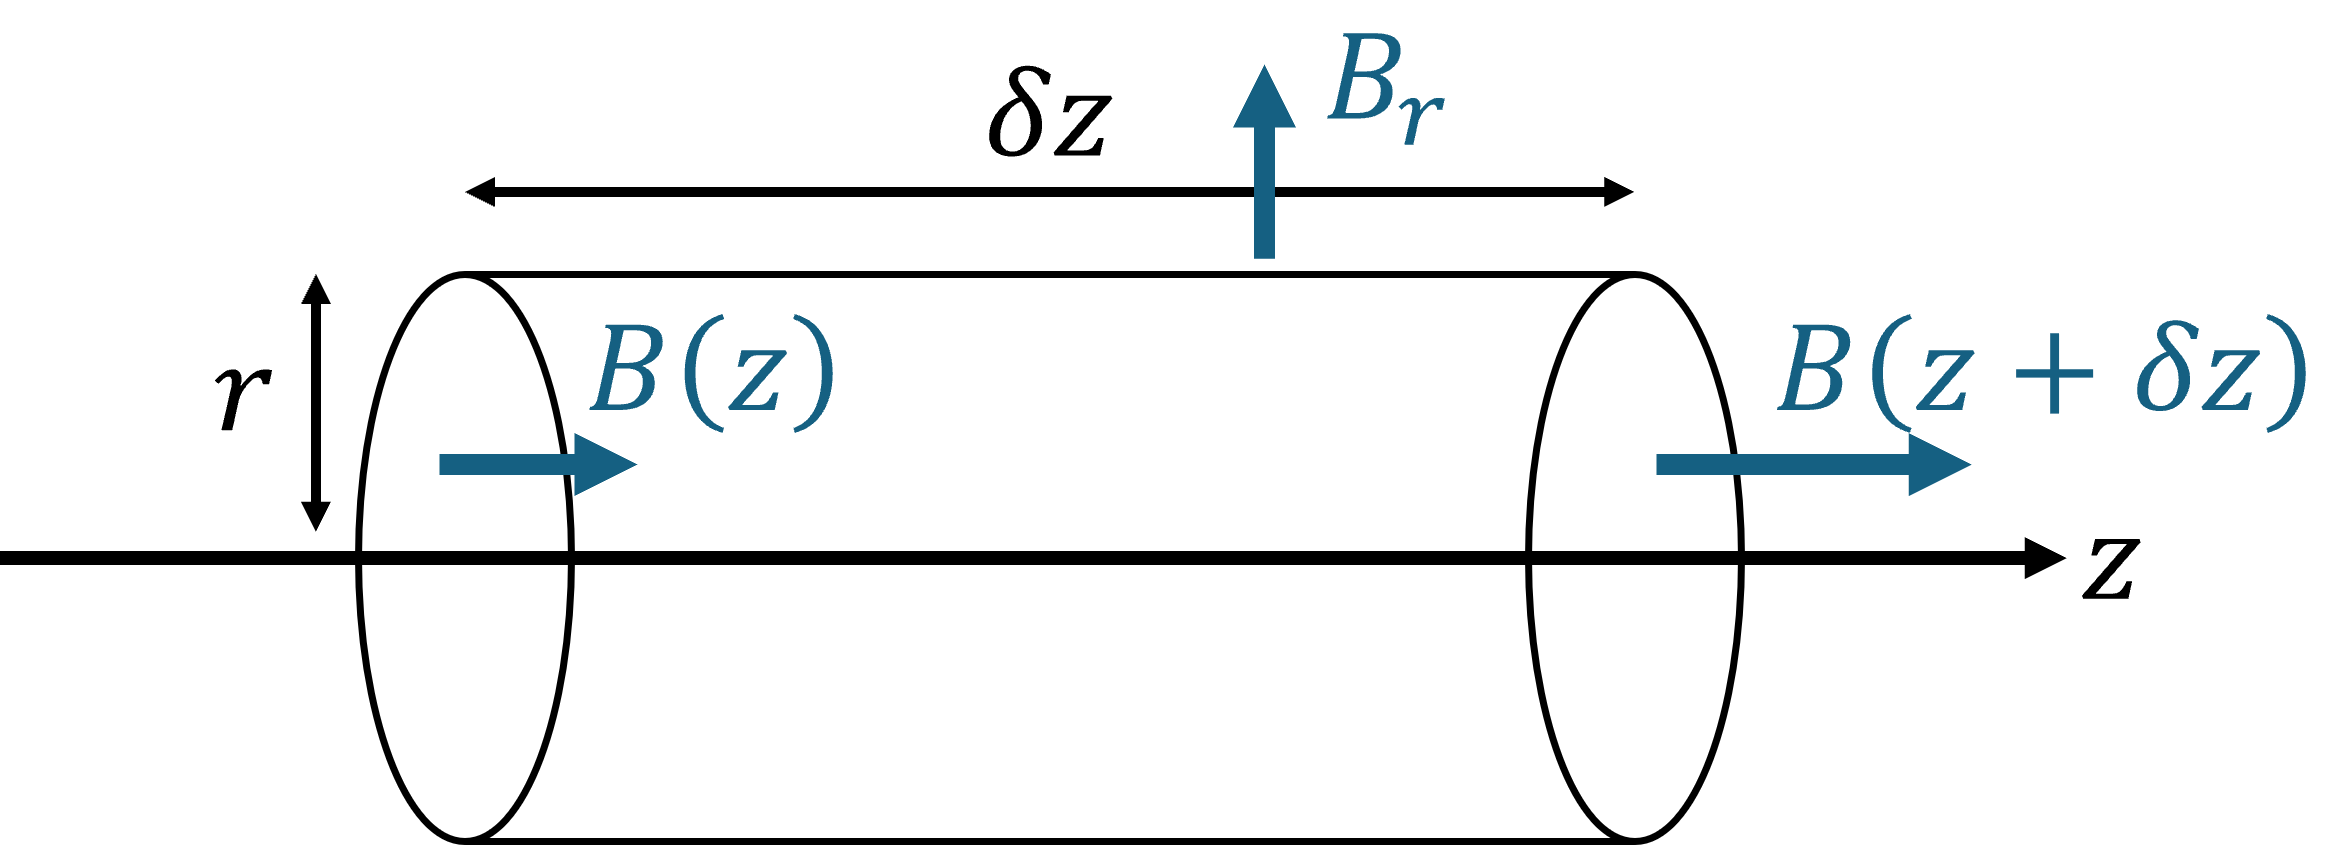
\includegraphics[width=0.5\linewidth]{Images/maxwell_2_cilinder.png}
    \caption{We kunnen de tweede Maxwell gebruiken om een relatie te vinden tussen $B_r$ en $B(z)$ op de symmetrie-as van het systeem. We tekenen daarvoor een cilindervormig Gauss-oppervlak waardoor de totale flux $\int\mathbf{B}\cdot d\mathbf{S}$ moet verdwijnen.}
    \label{fig:maxwell_2_cilinder}
\end{figure}
De flux doorheen de mantel wordt gegeven door $2\pi r\delta zB_r$, terwijl de flux doorheen het boven-en ondervlak gegeven wordt door $\pi r^2(B(z+\delta z)-B(z)\approx\pi r^2\frac{dB}{dz}$. Hieruit volgt:
\begin{equation}\label{eq:Br_Bz_relation}
    \int_S\mathbf{B}\cdot d\mathbf{S}=\pi r^2\frac{dB}{dz}+2\pi r\delta zB_r=0\Leftrightarrow B_r=-\frac{1}{2}r\frac{dB}{dz}
\end{equation}
Invullen van \ref{eq:Br_Bz_relation} in \ref{eq:theta_tussenstap} geeft:
\begin{equation}
    \frac{d}{dt}\left(mr^2\frac{d\theta}{dt}\right)=er\left(B\frac{dr}{dt}+\frac{1}{2}r\frac{dB}{dz}\frac{dz}{dt}\right)=\frac{d}{dt}\left(\frac{1}{2}er^2B\right)
\end{equation}
Beide leden integreren\footnote{In principe moet hier nog een constante $+C$ bij, maar aangezien $\frac{d\theta}{dt}=0$ bij $\mathbf{B}=0$ is $C=0$.} en vereenvoudigen geeft:
\begin{equation}\label{eq:precession}
    \frac{d\theta}{dt}=\frac{eB}{2m}=\eta^2B
\end{equation}
met $\eta=\sqrt{\frac{e}{2m}}\approx3\times10^5\sqrt{\frac{Q}{kg}}$ voor elektronen. We kunnen nu vergelijking \ref{eq:precession} invullen in vergelijking \ref{eq:2nd_law_newton_r}:
\begin{equation}\label{eq:paraxialevgl_dt}
    \frac{d^2r}{dt^2}=-r\frac{e^2B(z)^2}{2m^2}+r\frac{e^2B(z)^2}{4m^2}=-\eta^4B(z)^2r
\end{equation}
Nu willen we nog de variabele $t$ vervangen door $z$ om zo een gewone differentiaalvergelijking in 1 variabele te krijgen. Stel dat we werken met een versnelspanning $\Phi$, dan geldt er wegens behoud van energie dat:
\begin{equation}
    \frac{1}{2}m\left(\frac{dz}{dt}\right)^2=e\Phi\Leftrightarrow\frac{dz}{dt}=\sqrt{\frac{2e\Phi}{m}}=2\eta\sqrt{\Phi}
\end{equation}
Waaruit volgt:
\begin{equation}
    \frac{d^2}{dt^2}=4\eta^2\Phi\frac{d^2}{dz^2}
\end{equation}
Door dit in te vullen in \ref{eq:paraxialevgl_dt} komen we uiteindelijk bij de paraxiale bewegingsvergelijking voor axissymetrisch magnetisch veld:
\begin{equation}\label{eq:paraxialevgl}
    \frac{d^2r}{dz^2}+\frac{\eta^2B(z)^2}{4\Phi}r=0
\end{equation}
De relativistisch correcte versie van deze vergelijking is:
\begin{equation}\label{eq:paraxialevgl_rel}
    \frac{d^2r}{dz^2}+\frac{\eta^2B(z)^2}{4V}r=0
\end{equation}
Met $V=\Phi\left(1+\frac{e}{2mc^2}\Phi\right)$. Deze vergelijking zullen we later numeriek oplossen voor het geschatte magnetisch veld om de lenseigenschappen van lenzen te simuleren. \\

Merk op dat de paraxiale bewegingsvergelijking lineair is. Dit betekent dat twee lineair onafhankelijke oplossingen voldoende is om de algemene oplossing van deze vergelijking op te stellen. Conventioneel noemt men $z_0$ de positie van het vlak van het voorwerp dat we met een magnetische lens willen uitvergroten, en kiest met twee basisoplossingen $g(z)$ en $h(z)$ zodanig dat:
\begin{align}
    g(z_0)=1, g'(z_0)=0 \\[6pt]
    h(z_0)=0, h'(z_0)=1
\end{align}
Merk op dat de oplossing $g$ het gedrag van een parallelle bundel beschrijft. Immers, de oplossing voor de paraxiale bewegingsvergelijking van een parallel elektron dat initieel op een constante afstand $r_0$ van de optische as beweegt kan geschreven worden als $r_0g(z)$. Stel dat $g(z)$ een nulpunt heeft, dan kruisen alle initieel parallel bewegende elektronen de optische as in dat nulpunt. Dit is exact de gewenste werking van een magnetische elektronenlens; het nulpunt van $g(z)$ is dan het brandpunt van de lens. Vergelijking \ref{eq:paraxialevgl_rel} lijkt erg op een harmonische oscillator (met een frequentie afhankelijk van $B^2$), wat betekent dat de elektronen steeds naar de optische as worden afgebogen. In het algemeen zal $g(z)$ daarom altijd een nulpunt hebben als $B(z)\neq0$.
\section{Mesh shadowgraph methode}
Om de focale lengte en eventueel andere lenseigenschappen van de lens te bepalen gebruiken we een aangepaste versie van de \textit{rear mesh shadowgraph methode} beschreven in \cite{meshshadowgraphs}. Het algemene principe van deze methode bestaat er in om met behulp van de lens een divergerende elektronenbundel te maken. De focale lengte kan dan worden afgeleid door te meten hoe divergent deze elektronenbundel juist is. Concreet kunnen we dit meten door een fijnmazig rooster (mesh grid) achter de lens in de divergerende bundel te plaatsen, zodat er een uitvergroot schaduwbeeld op de detector wordt geworpen. De magnificatie van het schaduwbeeld is dan een maat voor de divergentie van de elektronenbundel. Hieronder werken we enkele gevallen wiskundig uit.\\

Een van de methodes beschreven in \cite{meshshadowgraphs} maakt gebruik van een puntbron op de optische as die we een afstand $z>f$ van de lens plaatsen. We veronderstellen dat we een dunne lens gebruiken, waardoor we de dunne lensformule kunnen gebruiken:
\begin{equation}\label{eq:thin_lens_formula}
    \frac{1}{f}=\frac{1}{z}+\frac{1}{z'}
\end{equation}
De puntbron wordt dan achter de lens afgebeeld op een afstand $z'>f$ van de lens. We plaatsen nu een grid met een nauwkeurig gekende periode van $e_1$ op een afstand $b$ van de lens, waarbij $b>z'$ zodat de elektronenbundel wordt gefocusseerd voor het grid. Op een afstand $d$ van het grid plaatsen we een elektronendetector. Het beeld van de puntbron op $z'$ veroorzaakt nu een divergerende elektronenbundel die een uitvergroot schaduwbeeld van het grid op de detector werpt. De opstelling wordt getoond op Figuur \ref{fig:rear_mesh_shadowgraph}.
\begin{figure}[H]
    \centering
    
\includegraphics[width=0.6\linewidth]{Images/rear_mesh_shadowgraph.png}
    \caption{Rear mesh shadowgraph methode voor een puntbron voor het focaalvlak van de lens. Door de magnificatie $M=\frac{E}{e}$ te meten is het mogelijk om het beeldpunt $z'$ en de focale lengte $f$ te bepalen.}
    \label{fig:rear_mesh_shadowgraph}
\end{figure}
Op het detectorbeeld meten we de grootte van 1 of meerdere afgebeeldde roosteropeningen, welke we aanduiden met $E$. De werkelijke afmeting van de roosteropeningen duiden we aan met $e=ne_1$ met $n$ het aantal roosteropeningen dat we beschouwen. De magnificatie van het schaduwbeeld is gelijk aan $M\frac{E}{e}$. Uit gelijkvormigheid van driehoeken volgt dan:
\begin{equation}
    \frac{c}{e}=\frac{c+d}{E}\Leftrightarrow\frac{E}{e}=M=1+\frac{d}{c}
\end{equation}
Dit kunnen we omvormen om $c$ te vinden:
\begin{equation}
    c=\frac{d}{M-1}
\end{equation}
Hiermee kunnen we eenvoudig de beeldafstand $z'$ bepalen:
\begin{equation}\label{eq:image_dist_real}
    z'=b-c=b-\frac{d}{M-1}
\end{equation}
Met de beeldafstand kunnen we de focaalafstand berekenen door vergelijking \ref{eq:thin_lens_formula} om te vormen. In het experiment dat we in deze thesis zullen uitvoeren passen we de voorgaande methode op twee manieren aanpassen, welke hieronder in meer detail worden uitgelegd.\\

Het is mogelijk dat de werkelijke focale lengte van de lens groter is dan de voorspelde focale lengte, waardoor de initiële puntbron achter het voorste focaalvlak van de lens ligt. In dat geval wordt er geen reëel beeld achter de lens, maar een virtueel beeld voor de lens gevormd. Dit wordt getoond op Figuur \ref{fig:rear_mesh_shadowgraph_virtual}.
\begin{figure}[H]
    \centering
    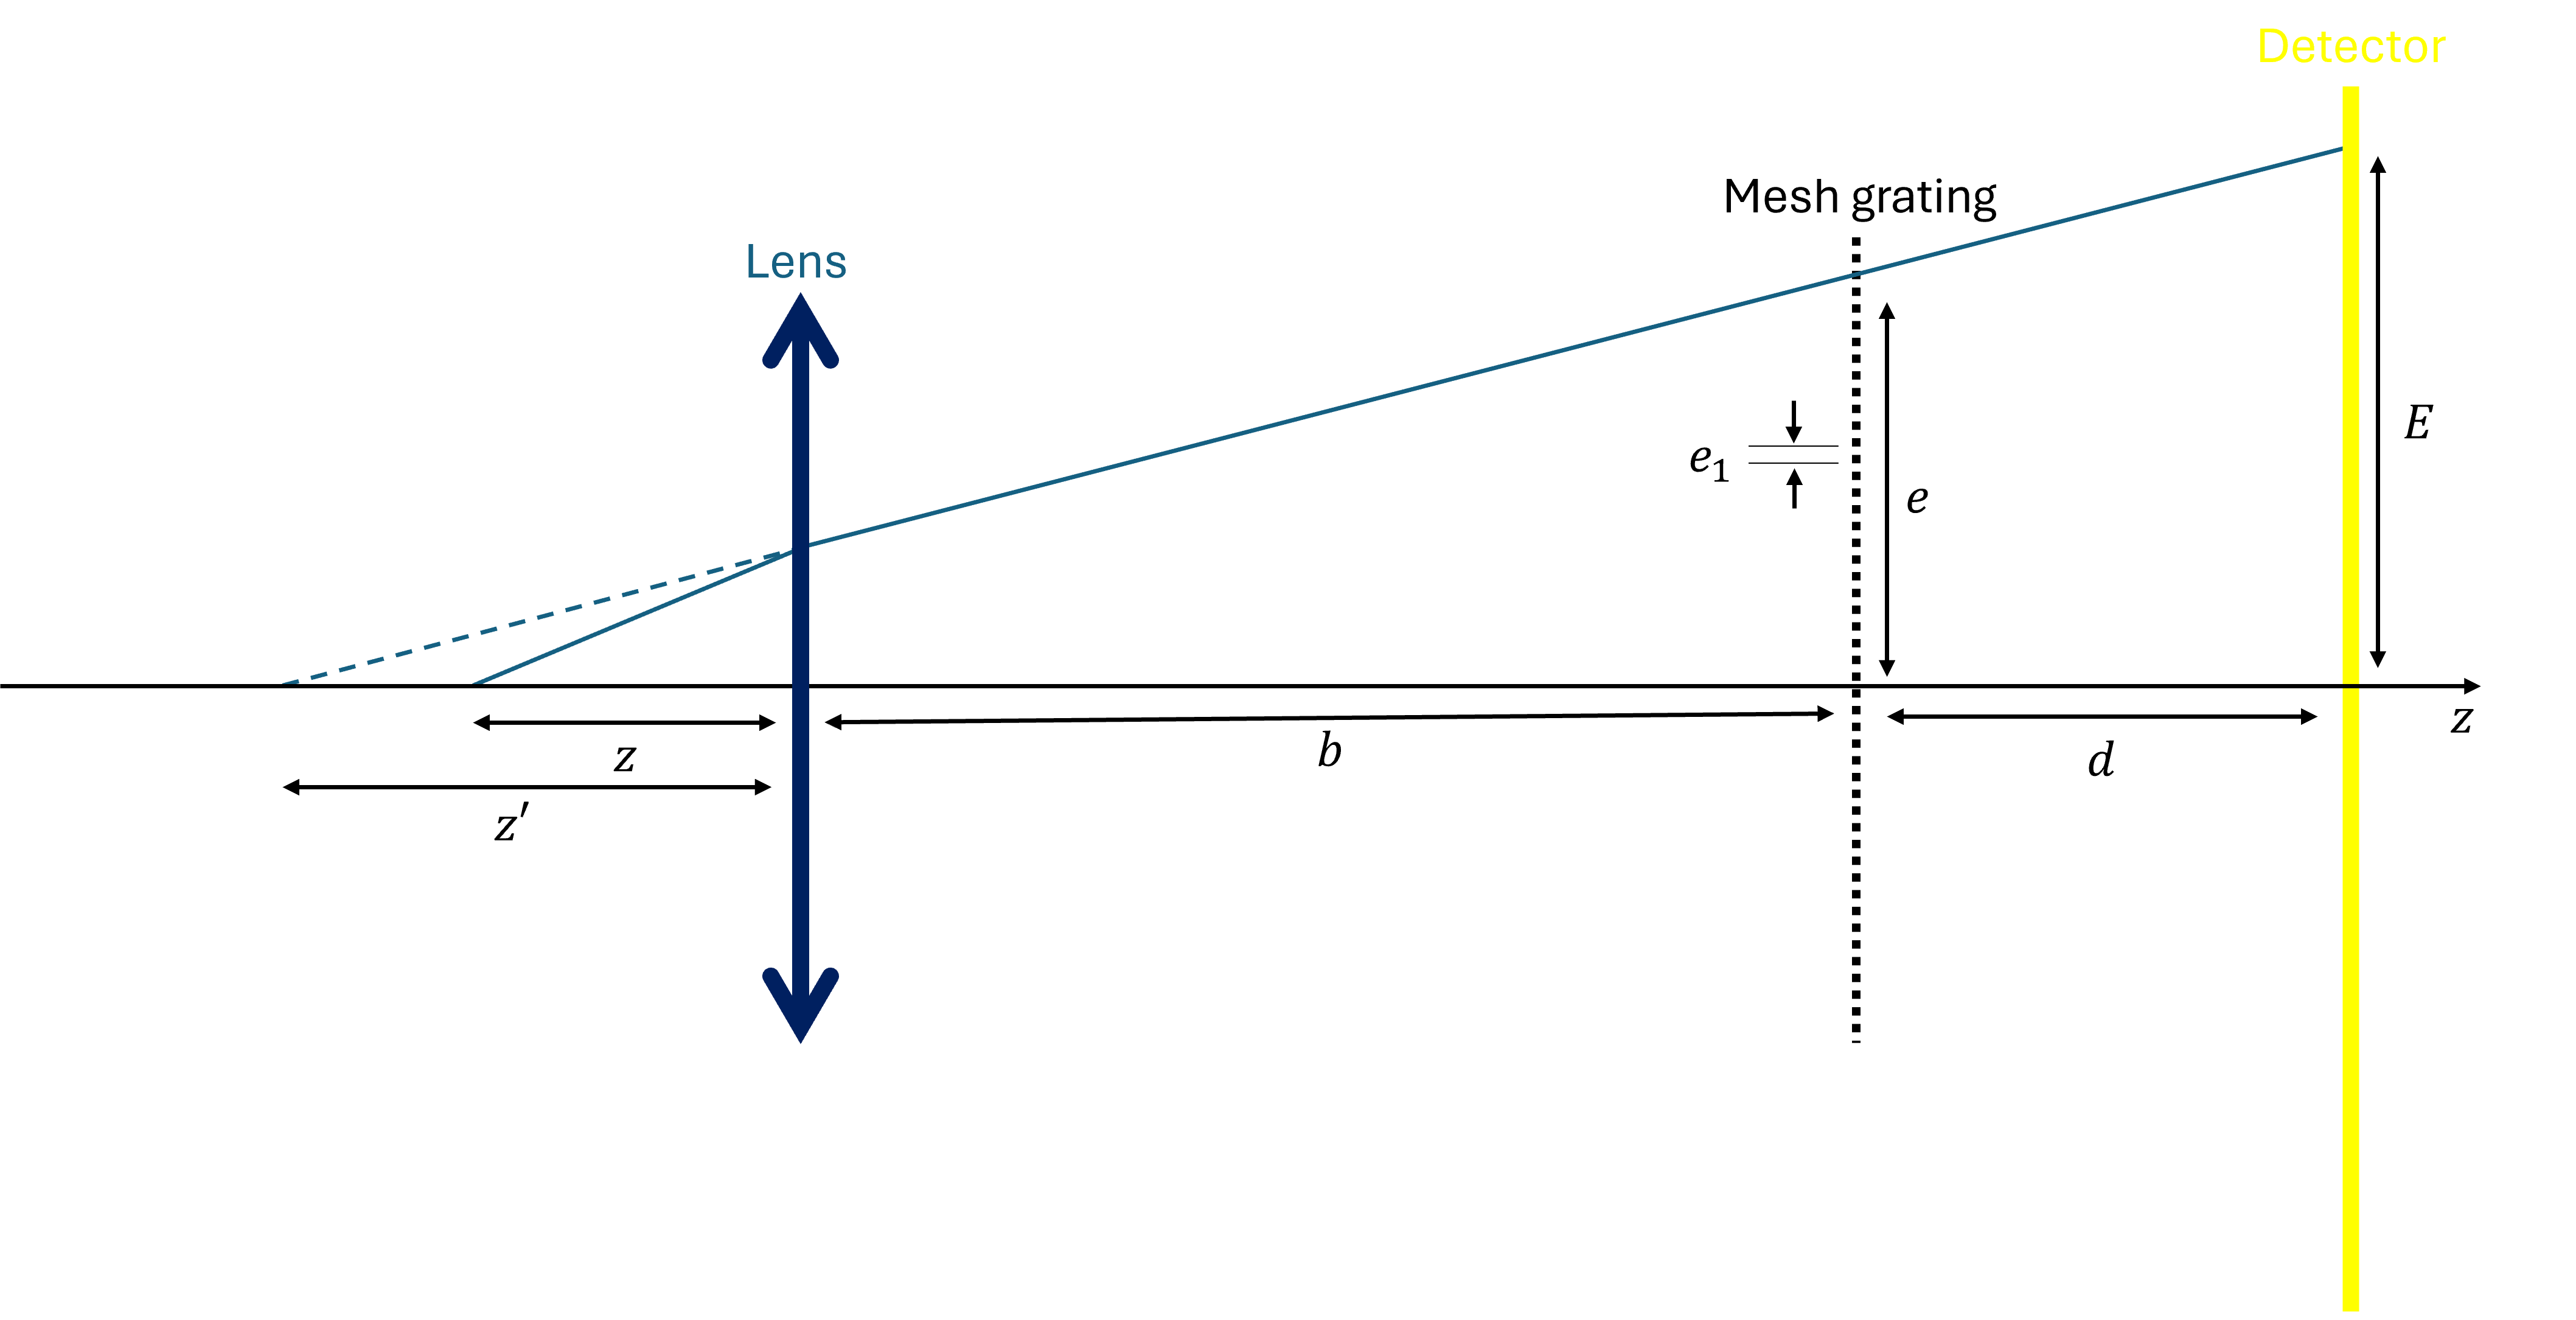
\includegraphics[width=0.6\linewidth]{Images/rear_mesh_shadowgraph_virtual_image.png}
    \caption{Rear mesh shadowgraph methode voor een puntbron achter het focaalvlak van de lens. De elektronenbundel wordt nu niet gefocusseerd in een punt, maar de elektronenbundel is nog steeds divergerend wat een magnificatie $M>1$ geeft. }
    \label{fig:rear_mesh_shadowgraph_virtual}
\end{figure}
Het is met deze opstelling nog steeds mogelijk om op deze manier de focale lengte te berekenen. Opnieuw vinden we uit gelijkvormigheid dat:
\begin{equation}
    \frac{e}{z'+b}=\frac{E}{z'+c+d}\Leftrightarrow\frac{E}{e}=M=1+\frac{d}{z'+b}
\end{equation}
Dit omvormen naar $z'$ geeft:
\begin{equation}
    z'=b-\frac{d}{M-1}
\end{equation}
Merk op dat dit exact dezelfde formule geeft als bij een reëel beeld (\ref{eq:image_dist_real}). Opnieuw gebruiken we \ref{eq:thin_lens_formula} om $f$ te berekenen.\\

Een mogelijke manier om de mesh shadowgraph methode te vereenvoudigen is om een paralelle i.p.v. een conische elektronenbundel op de lens in te sturen. In dat geval is $z=\infty$, waardoor uit \ref{eq:thin_lens_formula} volgt dat $z'=f$. We kunnen dezelfde procedure als in de originele methode gebruiken om $c$ te bepalen, maar nu kunnen we de focale lengte rechtstreeks bepalen uit $f=b-c$. Figuur \ref{fig:rear_mesh_shadowgraph_parallel} toont de opstelling in dit geval.
\begin{figure}[H]
    \centering
    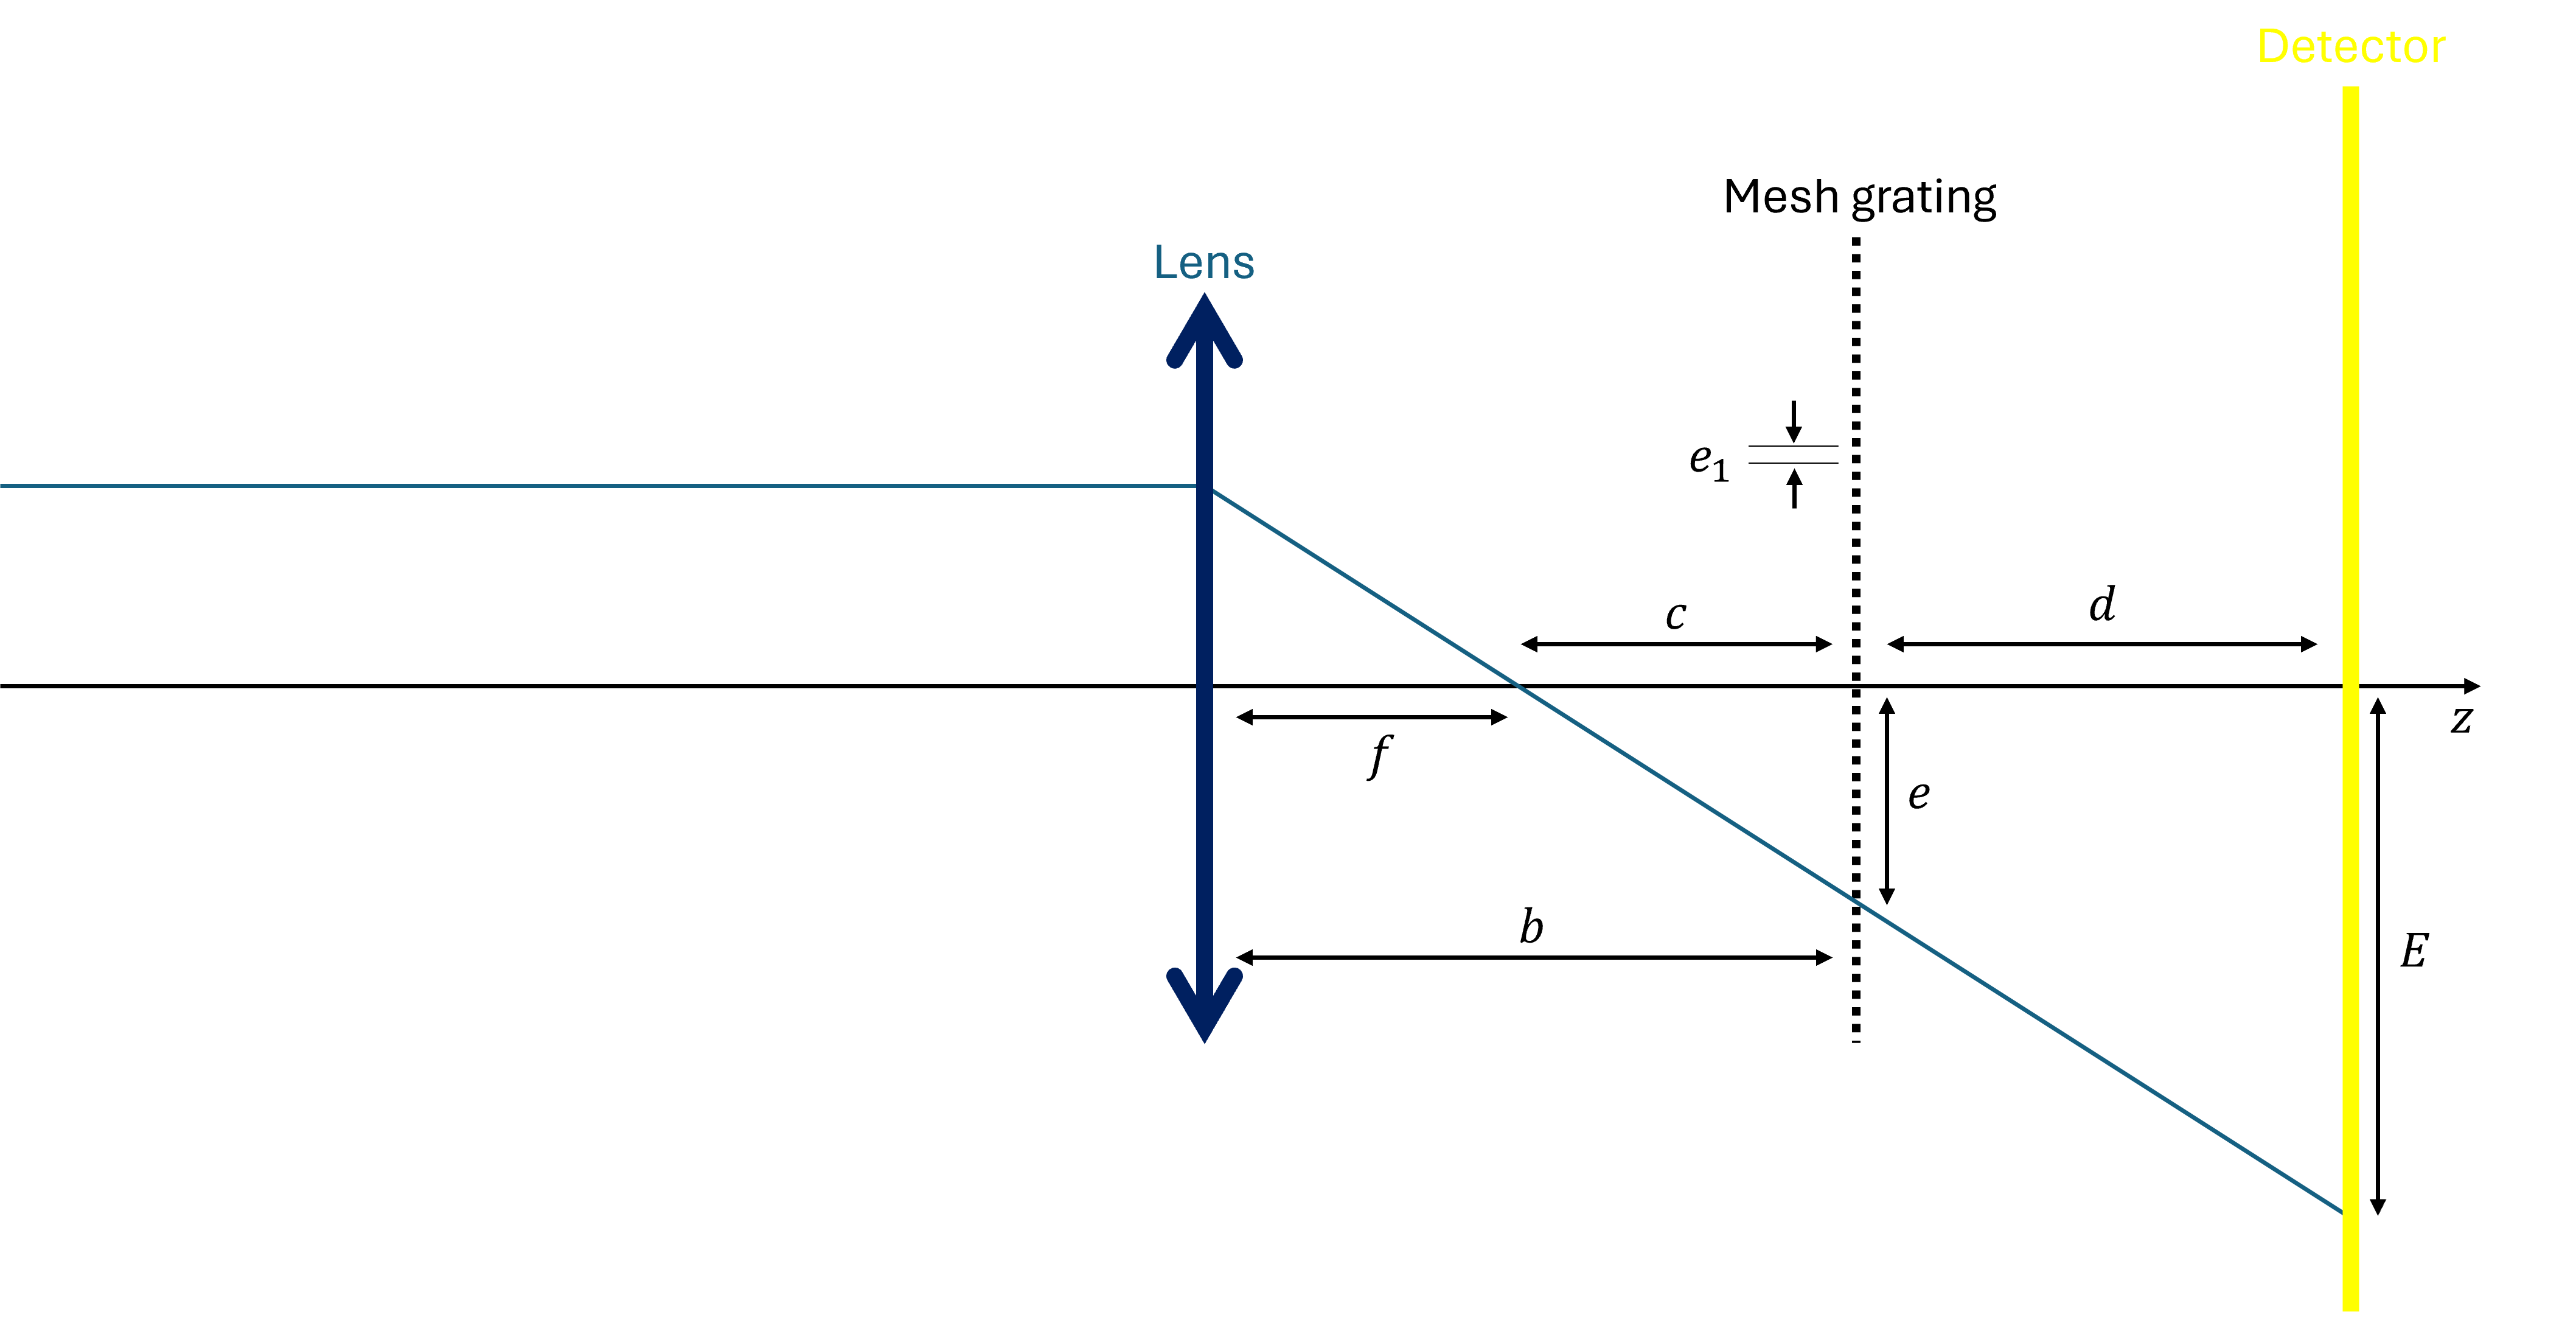
\includegraphics[width=0.6\linewidth]{Images/rear_mesh_shadowgraph_parallel_beam.png}
    \caption{Rear mesh shadowgraph methode voor een parallelle bundel. Door het gebruik van een parallelle bundel worden de inkomende elektronenbundels door de lens gefocusseerd in het focaalvlak achter de lens, wat de bepaling van de focale lengte iets vereenvoudigt.}
    \label{fig:rear_mesh_shadowgraph_parallel}
\end{figure}
In principe kan deze methode ook uitgebereid worden om de chromatische en sferische abberatiecoëfficienten van de lens te berekenen. De sferische abberatiecoëfficient kan worden afgeleid door de afgebeeldde grootte van de individuele roosteropeningen uit te zetten in functie van de afstand tot de optische as van het systeem. Immers, hoe verder de roosteropening zich van de optische as bevindt, hoe groter de hoek $\alpha$ tussen de elektronen en de optische as. Sferische abberatie kan worden uitgedrukt als $\Delta z' = -C_s \alpha^2$, dus door $z'$ voor verschillende waarden van $\alpha$ te berekenen kunnen we de sferische abberatiecoëfficient $C_s$ fitten. De chromatische abberatie kunnen we berekenen door de versnelspanning van de micrscoop aan te passen. De chromatische abberatiecoëfficient $C_f$ kunnen we dan berekenen uit $\frac{\Delta f}{f}=C_f\frac{\Delta V}{V}$.

\chapter{Eigen realisatie}
\section{Werking permanente magneetlens}
Voor we in de details van het ontwerpsproces van de lens duiken, is het verstandig om het concept van het ontwerp helder uit te leggen. Het doel is om een magnetisch veld te ontwerpen dat de elektronen op zo'n manier afbuigt zodanig dat een paralelle bundel geconcentreerd zal worden in een punt op de optische as. Hierbij willen we dat de lens aan enkele gewenste eigenschappen voldoet.\\

Ten eerste willen we een geschikte focale lengte zodat de lens bruikbaar is in een elektronenmicroscoop. Concreet zal deze lens getest worden in een Tescan MIRA SEM, waarin we een maximale totale afstand van $228.4\mathrm{mm}$ van elektronenbron tot detector ter beschikking hebben. Om een bruikbare lens te maken is het daarom gewenst dat de focale lengte niet veel langer dan $10\mathrm{mm}$ is. Verder zullen we werken we met een versnelspanning van $30\mathrm{KeV}$, wat een voorwaarde legt op de minimale sterkte van het magnetisch veld. \\

%% Meer uitleg over wat een hoofdvlak is?
Ten tweede is het gewenst dat de lens die we maken, een dunne lens is. Meer concreet willen we dat de hoofdvlakken samenvallen in het midden van de lens. Op deze manier is het gemakkelijker om berekeningen te doen als we opstellingen met meerdere lenzen willen bouwen, aangezien de dunne lensformule dan toepasbaar is. Dit betekent dat we een sterk ruimtelijk geconcentreerd magnetisch veld in het midden van de lens willen; de elektronen interageren dan maar heel kort met het magnetisch veld, wat een dunne lenswerking geeft. Hoe geconcentreerder we het veld maken, hoe sterker het maximale veld moet zijn om dezelfde afbuiging te veroorzaken. Om een bruikbare lens te maken willen we op de optische as een magnetisch veld met een sterkte van $\sim0.1-1\mathrm{T}$ dat geconcentreerd is over een afstand van $<5\mathrm{mm}$. \\

Het ontwerp dat we in deze thesis onderzoeken en aan beide voorwaarden voldoet, wordt getoont op Figuur \ref{fig:lens_circuit_diagram}.
\begin{figure}[H]
    \centering
    
\includegraphics[width=0.6\linewidth]{Images/lens_circuit_diagram.png}
    \caption{Cross-sectie van het ontwerp van onze permanente magneetlens. Een homogeen gemagnetiseerde Nd-ringmagneet maakt een sterk magnetisch veld dat door twee zacht magnetische polepieces wordt geconcentreerd in het  het gat van de lens.}
    \label{fig:lens_circuit_diagram}
\end{figure}

Om een axissymetrisch veld te veroorzaken, maken we gebruik van een kleine ringvormige NdFeB magneet met een remanent magneetveld van $\sim1.4\mathrm{T}$. We kunnen in principe enkel de magneet als lens gebruiken, maar dit is niet optimaal; het magnetisch veld zou dan uitgebreid in de ruimte zijn, terwijl we een zo sterk mogelijk veld op de symmetrieas van de lens willen. We kunnen het veld naar het midden van de lens "begeleiden" d.m.v. polepieces gemaakt uit een zacht ferromagnetisch materiaal met een hoge permeabiliteit $\mu$. Als de permabiliteit voldoende hoog is, dan zullen de grote meerderheid van de veldlijnen in de polepieces blijven en in het midden van de lens de opening of \textit{gap} oversteken. Bij het oversteken van de opening tussen de polepieces lopen de velden niet perfect loodrecht van het ene oppervlak naar het andere, maar door randeffecten zullen ze naast de oppervlakken naar buiten buigen. Op deze manier krijgen we in het gat een lokaal sterk veld, zoals gewenst.
\section{Analytische afschatting magnetisch veld}
Vooraleer we de lenseigenschappen van de lens kunnen simuleren, willen we een analystische schatting maken van het magnetisch veld $B(z)$ op de symmetrieas van de lens. Hiervoor maken enkele belangrijke benaderingen om de berekeningen te vereenvoudigen.\\

Ten eerste veronderstellen we dat de magnetische veldlijnen volledig in de polepieces zullen blijven tot ze de gap tussen de polepieces bereiken, zonder dat er magetisch veld op andere plaatsen naar buiten lekt. We zorgen ervoor dat dit een goede benadering blijft door de geometrie van de polepieces zo te ontwerpen dat het magnetisch veld nergens anders kan kortsluiten. We willen met andere woorden dat er geen andere paden $C$ van de bovenkant naar de onderkant van de ringmagneet mogelijk zijn die een een kleinere/gelijkaardige reluctantie $\mathcal{R}=\int_C\frac{dl}{\mu(l)A(l)}$ hebben. Daarnaast zorgen we ervoor dat de polepieces gladde en afgeronde oppervlakken hebben om randeffecten te voorkomen, aangezien magnetische veldlijnen de neiging hebben om zich te concentreren rond oppervlakken met een kleine kromtestraal, zoals randen en hoeken.\\

Om wiskundig te beschrijven waar de magnetische velden de polepieces verlaten of weglekken, is het gemakkelijk om gebruik te maken van magnetische poolladingen. De magnetische lading aan het oppervlak van een gemagnetiseerd volume wordt gegeven door $\sigma_M=\mathbf{M}\cdot\mathbf{n}$ met $\mathbf{M}$ de magnetisatie van het materiaal en $\mathbf{n}$ een normaalvector op het oppervlak. In het ideale geval zijn de polepieces zo gemagnetiseerd dat de magnetisatie altijd parallel ligtaan de zijoppervlakken ligt zodat $\sigma_M=0$. Alleen bij de oppervlakken die aan de gap grenzen staat de magnetisatie loodracht op het oppervlak, waardoor we daar wel een poollading krijgen. In deze benadering hebben de polepieces dus enkel oppervlakteladigen aan de gap tussen de polepieces.\\

Een tweede belangrijke veronderstelling is dat de poolladingen aan de oppervlakken in de gap homogeen verdeeld zijn. Dit is een goede benadering als we een homogeen ferromagnetisch materiaal en een homogeen gemagnetiseerde ringmagneet gebruiken. De oppervlakken van de ringmagneet kunnen we immers ook als homogeen geladen oppervlakken beschouwen. De magnetische veldlijnen afkomstig van het magneetoppervlak zullen zich min of meer uniform doorheen de polepieces voortplanten zodat ook de gap-oppervlakken homogeen geladen zijn. Op deze manier wordt het magnetisch veld gereduceerd tot het veld veroorzaakt door twee homogeen geladen \textit{annula}\footnote{Een annulus is een oppervlak opgespannen tussen twee concentrische cirkels.} met een tegengestelde, maar even grote magnetische poollading $\pm\sigma_M$.\\

Aan de hand van dit vereenvoudigd model kunnen we een analytische uitdrukking voor het magnetisch veld op de symmetrie-as terugvinden. We beginnen met 1 homogeen geladen annulus met een oppervlaktelading\footnote{Voorlopig kiezen we een arbitraire oppervlaktelading, in een latere sectie zullen we bespreken hoe we de juiste waarde voor $\sigma_M$ kiezen.} $+\sigma_M$ die zich rond de $z$-as op een hoogte $z=0$ bevindt. De annulus heeft een binnenstraal van $R_1$ en een buitenstraal $R_2$. Natuurlijk is het niet mogelijk om een magnetische monopool zoals in dit systeem te maken, maar dit is slechts een tussenstap: later zullen we een tweede annulus met tegengestelde lading toevoegen. Dit systeem wordt getoond op Figuur \ref{fig:analytic_expression_1_ring}.

\begin{figure}[H]
    \centering
    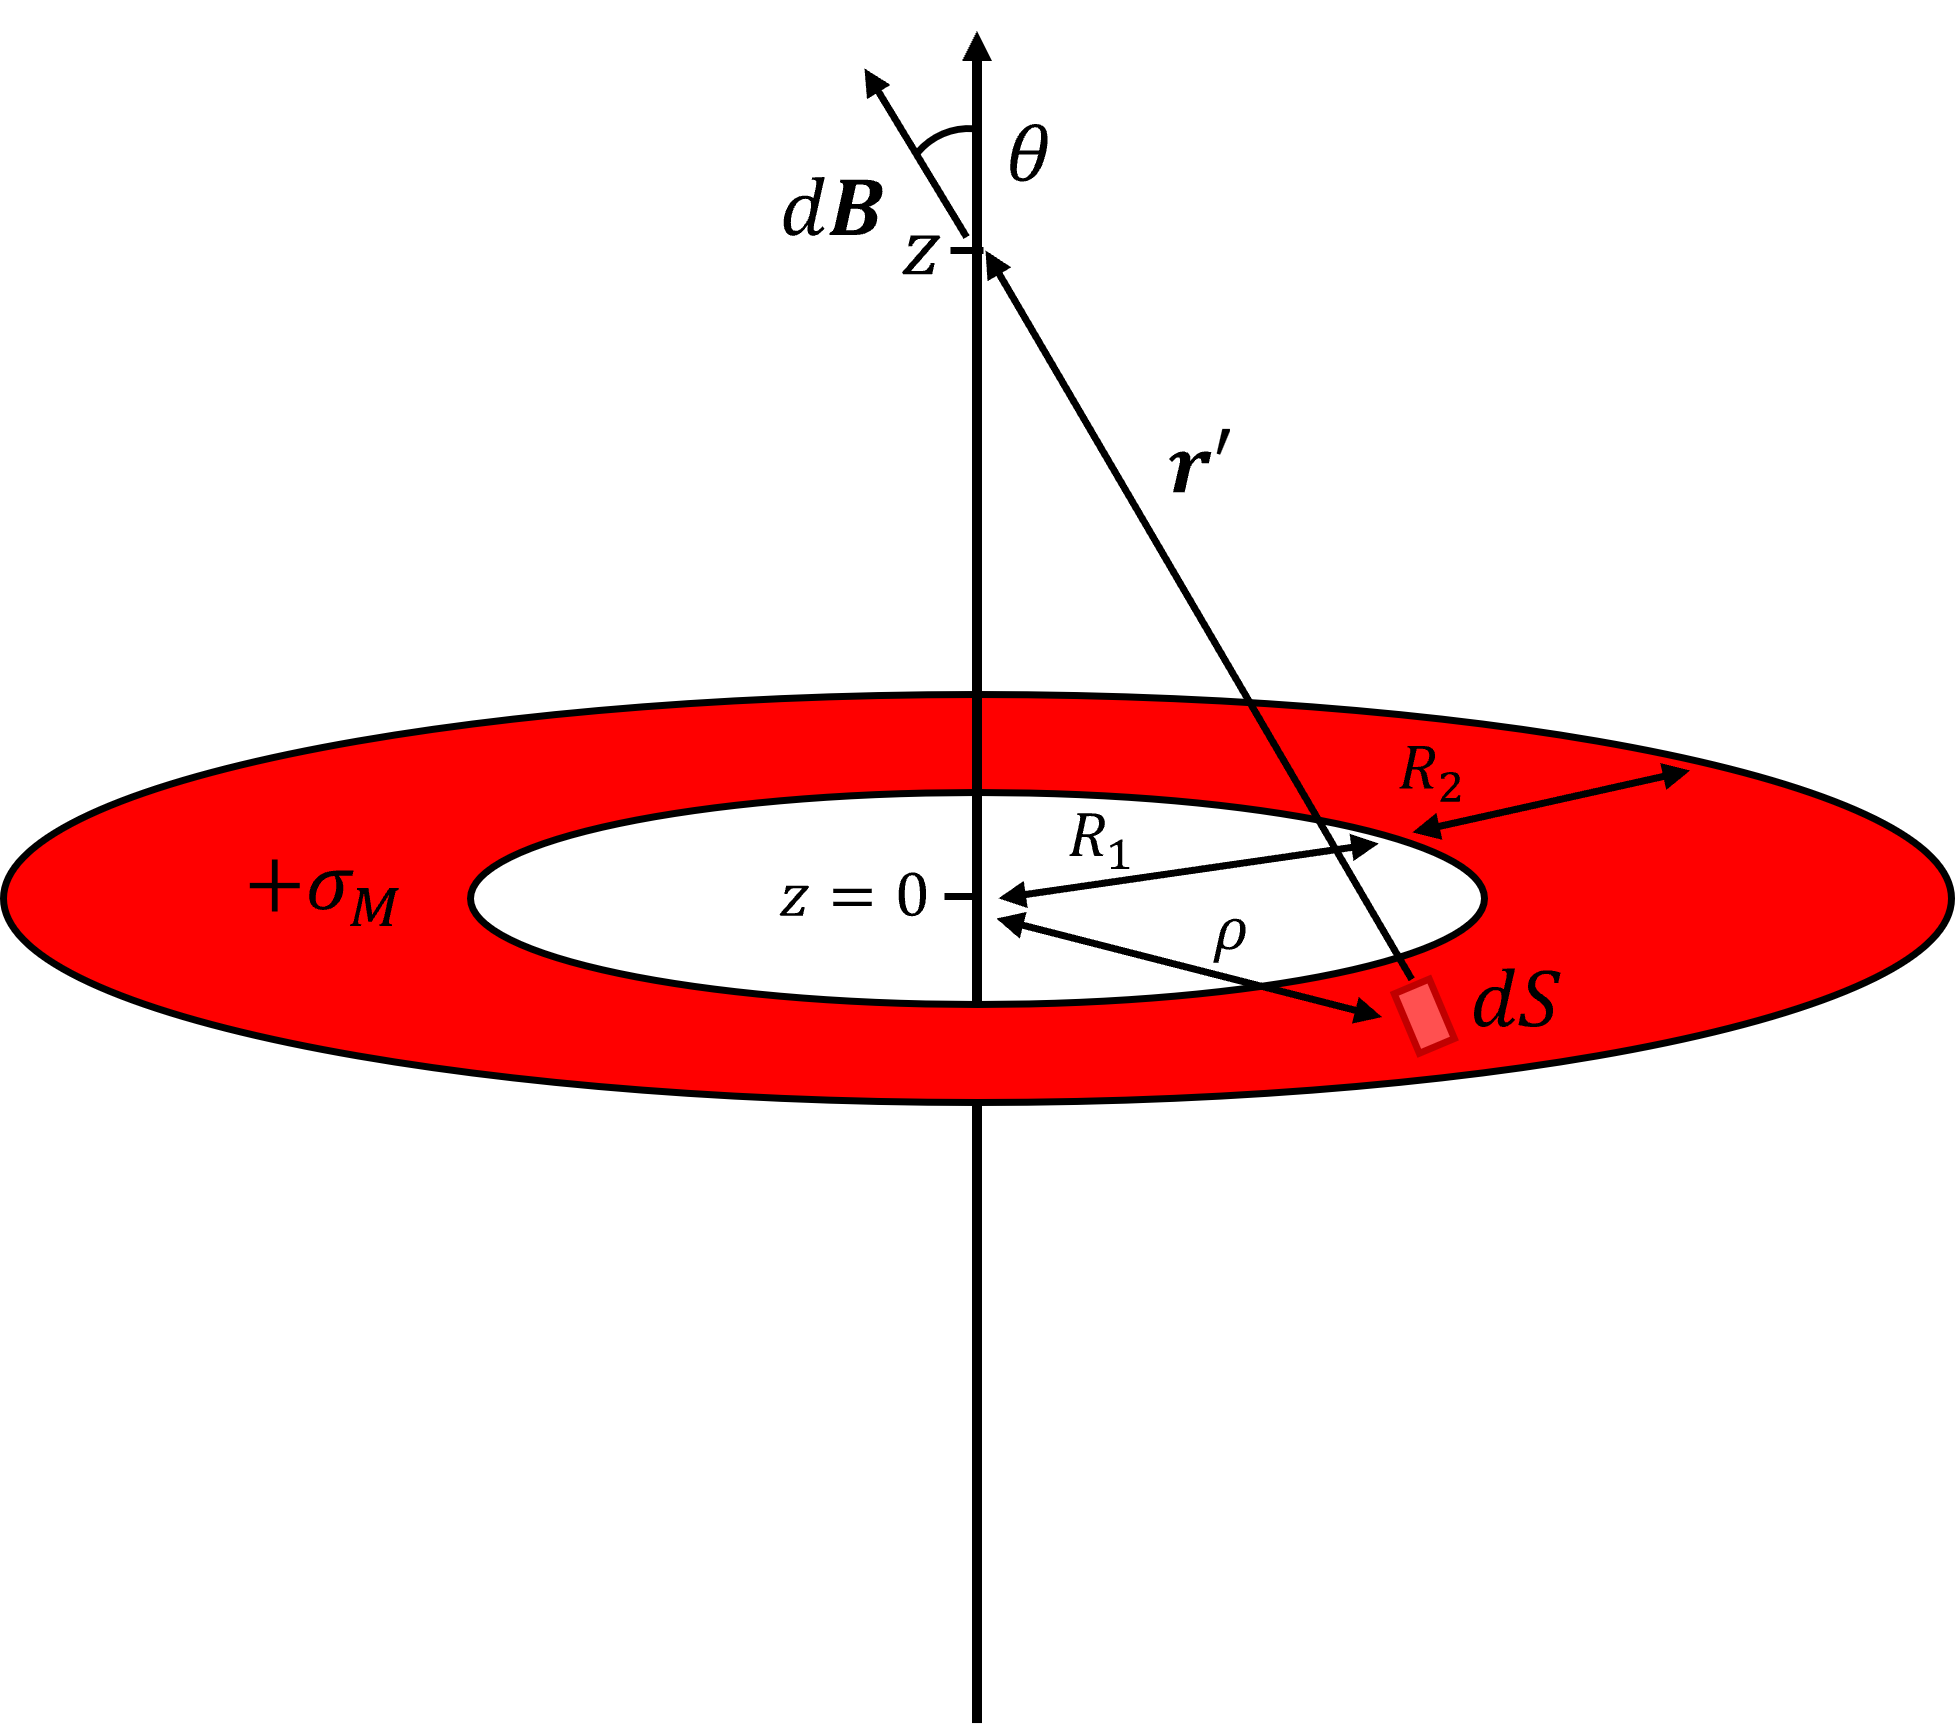
\includegraphics[width=0.5\linewidth]{Images/analytic_expression_1_ring.png}
    \caption{Systeem met 1 annulus rond een symmetrie-as. De annulus heeft een homogene oppervlaktepoollading gelijk aan $\sigma_M$, wat aanleiding geeft tot een magnetisch veld.}
    \label{fig:analytic_expression_1_ring}
\end{figure}

Het magnetisch veld in een bepaald punt $\mathbf{r}$ kan nu bepaald worden door de bijdragen van alle opeprvlakte-elementen van de annulus te integreren, net zoals we zouden doen in het elektrostatisch geval. We moeten enkel de permittiviteit $\epsilon$ vervangen door de permeabiliteit $\mu$. In ons geval zijn we enkel geïnteresseerd in het veld op de $z$-as, aangezien we in de paraxiale benadering zullen werken. Uit symmetrieoverwegingen kunnen we al zeggen dat enkel de component parallel met de $z$-as zal overblijven. We integreren de bijdragen van elk oppervlakte-elementje $dS$ op de annulus aan het resulterend magnetisch veld, dit resulteert in de volgende berekening:
\begin{equation} \label{eq:1_annulus}
\begin{split}
B_{ring}(z) & = \int_S\mathbf{e}_z\cdot d\mathbf{B} = \int_S\cos \theta\frac{ \mu_0\sigma_M}{4\pi|\mathbf{
r}'|^2}dS =  \frac{\mu_0\sigma_M}{4\pi}\int_S\frac{\cos \theta}{|\mathbf{r}'|^2}dS\\
& = \frac{\mu_0\sigma_M}{4\pi}\int_S\frac{\frac{z}{\sqrt{z^2+\rho^2}}}{z^2+\rho^2}dS = \frac{\mu_0\sigma_M}{4\pi} \int_0^{2\pi}d\phi \int_{R_1}^{R_2}\rho d\rho \frac{z}{(z^2+\rho^2)^{\frac{3}{2}}}\\
& = \frac{\mu_0\sigma_Mz}{2}\int_{R_1}^{R_2}\frac{\rho}{(z^2+\rho^2)^{\frac{3}{2}}}d\rho \quad \left(\text{Stel } u = z^2+\rho^2,\ du = 2\rho\, d\rho\right)\\
& = \frac{\mu_0\sigma_Mz}{4}\int_{z^2+R_1^2}^{z^2+R_2^2}u^{-\frac{3}{2}}du = \frac{\mu_0\sigma_Mz}{2}\left[-u^{-\frac{1}{2}}\right]_{z^2+R_1^2}^{z^2+R_2^2}\\
& = \frac{\mu_0\sigma_Mz}{2} \left(\frac{1}{\sqrt{z^2+R_1^2}}-\frac{1}{\sqrt{z^2+R_2^2}}\right)
\end{split}
\end{equation}
Op Figuur \ref{fig:B_field_1_annulus} tonen we een plot van $B_{ring}$ voor parameters $R_1=1$ en $R_2=2$. Zoals we zouden verwachten uit de symmetrie van het systeem is het veld 0 in het midden van de ring. Vlak boven en onder de ring neemt het veld sterk toe in de zin weg van de ring, aangezien veldlijnen weg van positieve/noordelijke poolladingen bewegen. Onder de ring is het veld negatief, aangezien we de $z$-as als positieve richting hebben gekozen. Ver weg van de ring kunnen we de ladingsverdeling als een puntlading beschouwen en valt het veld af als $\frac{1}{z}$.
\begin{figure}[H]
    \centering
    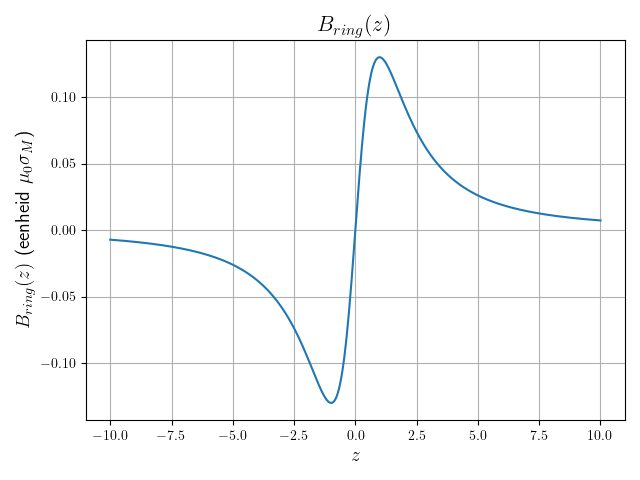
\includegraphics[width=0.6\linewidth]{Images/B_field_1_annulus.png}
    \caption{Plot van $B_{ring}$ volgens vergelijking \ref{eq:1_annulus} voor parameters $R_1=1$ en $R_2=2$. Het veld is antisymmetrisch rond het midden van de ring, zoals men zou verwachten.}
    \label{fig:B_field_1_annulus}
\end{figure}
Door te werken met poolladingsdichtheden kunnen we nu eenvoudig het veld met twee tegengesteld geladen ringvormige oppervlakken berekenen. We kunnen simpelweg een superpositie maken van twee velden veroorzaakt door een enkel oppervlak, aangezien elektromagnetische velden lineair zijn. Het systeem dat we nu beschrijven wordt getoont op Figuur \ref{fig:analytic_expression_2_rings}

\begin{figure}[H]
    \centering
    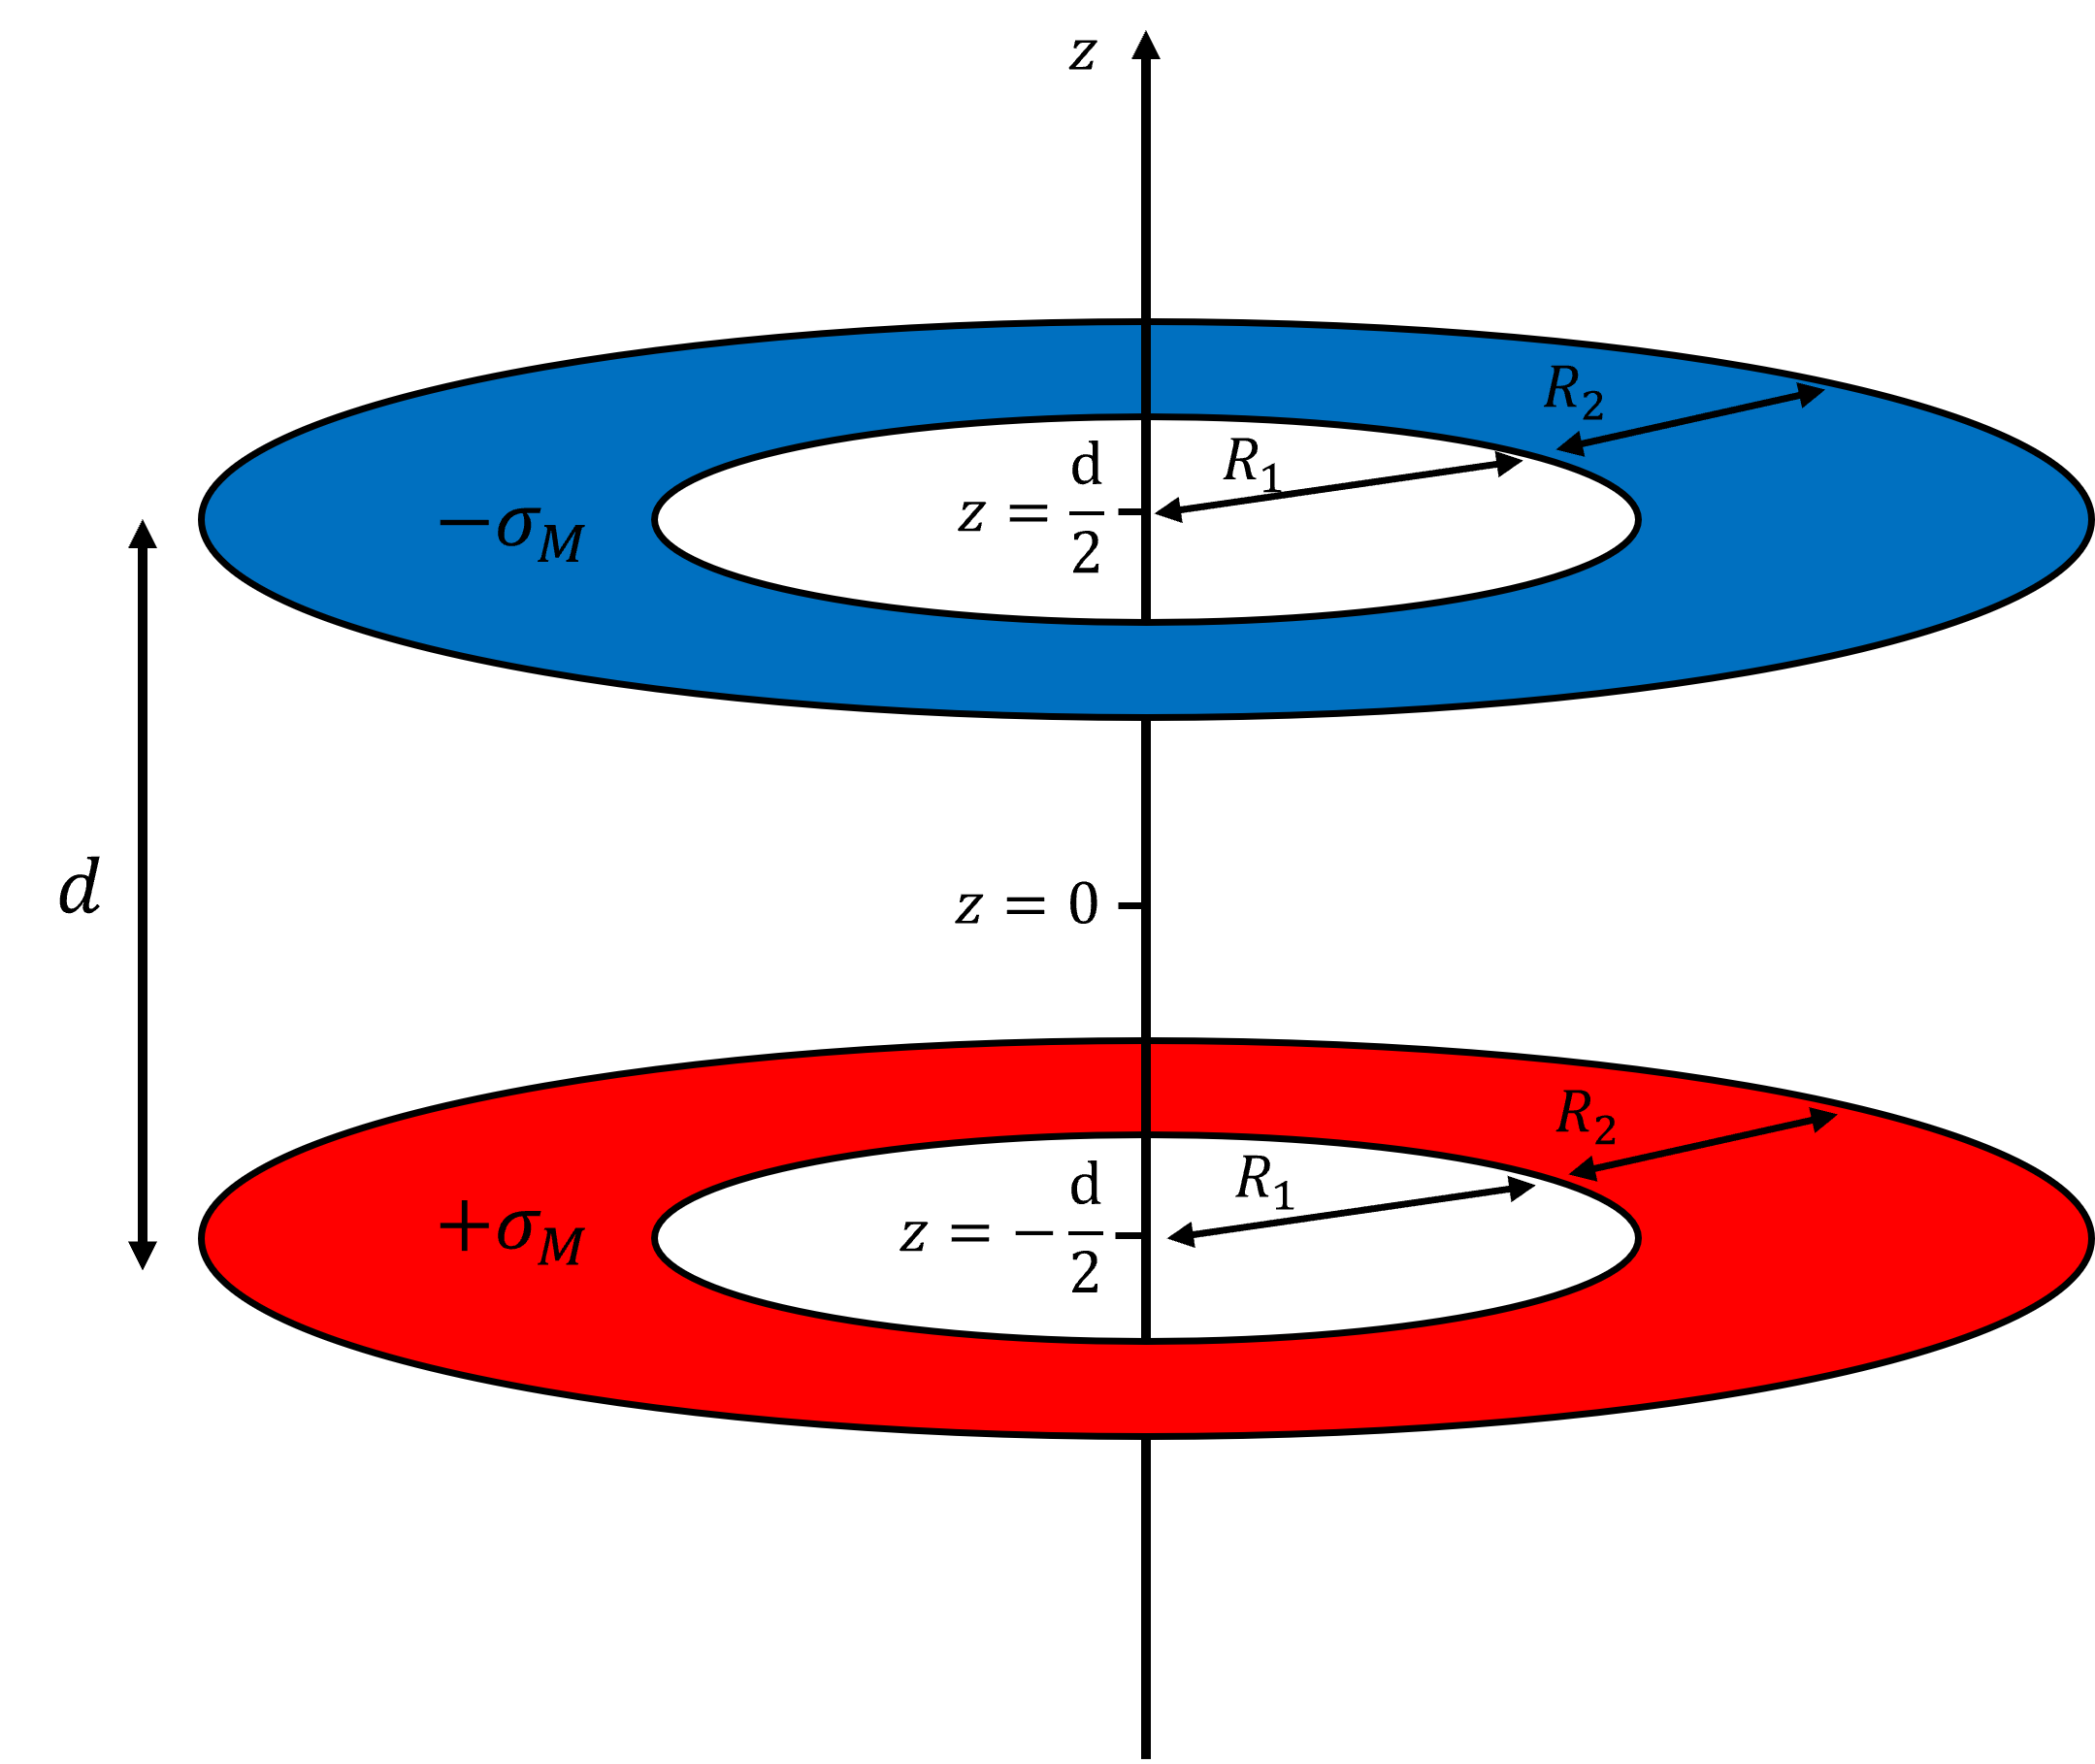
\includegraphics[width=0.45\linewidth]{Images/analytic_expression_2_rings.png}
    \caption{Systeem met 2 annula met een gapbreedte van $d$ rond een symmetrie-as. De annula hebben homogene oppervlaktepoolladingen gelijk aan $\pm\sigma_M$, wat aanleiding geeft tot een magnetisch veld. Dit is het systeem dat we beschouwen bij het afschatten van het magnetisch veld in onze lens.}
    \label{fig:analytic_expression_2_rings}
\end{figure}

Het magnetisch veld wordt nu gegeven door:
\begin{equation}\label{eq:2_annula}
\begin{split}
    B(z) & = B_{ring}\left(z+\frac{d}{2}\right)-B_{ring}\left(z-\frac{d}{2}\right)\\
    & = \frac{\mu_0\sigma_M\left(z+\frac{d}{2}\right)}{2}\left(\frac{1}{\sqrt{\left(z+\frac{d}{2}\right)^2+R_1^2}}-\frac{1}{\sqrt{\left(z+\frac{d}{2}\right)^2+R_2^2}}\right)-\frac{\mu_0\sigma_M\left(z-\frac{d}{2}\right)}{2}\left(\frac{1}{\sqrt{\left(z-\frac{d}{2}\right)^2+R_1^2}}-\frac{1}{\sqrt{\left(z-\frac{d}{2}\right)^2+R_2^2}}\right)
\end{split}
\end{equation}
Figuur \ref{fig:B_field_2_annula} toont een plot van onze analytische afschatting van $B(z)$ op de symmetrieas van de lens, met parameters $R_1=1$, $R_2=2$, $d=2$. 
\begin{figure}[H]
    \centering
    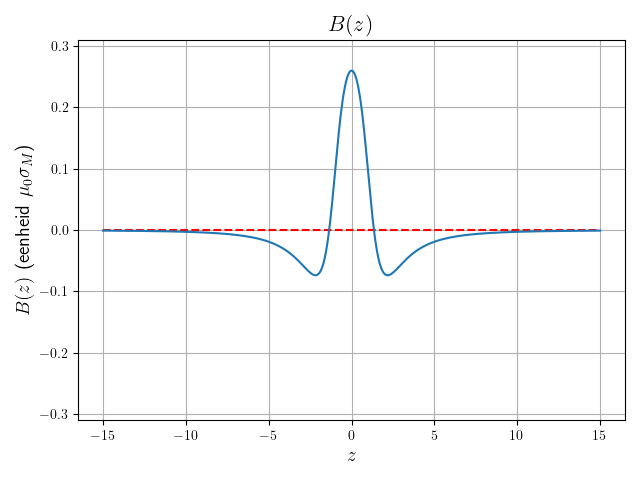
\includegraphics[width=0.6\linewidth]{Images/B_field_2_annula.png}
    \caption{Plot van $B$ volgens vergelijking \ref{eq:2_annula} voor parameters $R_1=1$, $R_2=2$, $d=2$. Het veld is nu symmetrisch rond het midden van de lens en maximaal in het midden van de lens, zoals men zou verwachten.}
    \label{fig:B_field_2_annula}
\end{figure}
We verkrijgen op deze manier een sterk gepiekt magnetisch veld in het midden van de lens. Dit is exact wat we willen om een dunne lens met een bruikbare focale lengte te maken. Later zullen we onderzoeken hoe de geometrie van de ringoppervlakken het magnetisch veld verandert, en hoe dit de lenseigenschappen beïnvloedt.\\

Een belangrijke opmerking bij deze afschatting is dat deze in principe enkel geldt in het gebied $-\frac{d}{2}<z<\frac{d}{2}$. De ringvormige ladingsoppervlakken zijn aan de buitenkanten immers begrensd door de polepieces, die een veel grotere permeabiliteit dan vacuüm hebben. In het ideale geval is het magnetisch veld geconcentreerd in de polepieces zonder dat het weglekt, en geldt er voor $z>\left|\frac{d}{2}\right|$ dat $B(z)=0$. Op bovenstaande figuur is echter te zien dat de velden buiten de lens heel wat kleiner zijn dan de velden in het centrum van de lens, en aangezien we in de paraxiale bewegingsvergelijkingen werken met $B^2$ zullen deze randvelden zeer weinig invloed hebben wanneer we de vergelijking numeriek zullen oplossen.\\

Onze analytische afschatting kunnen we numeriek controleren met het ionen- en elektronenoptica simulatieprogramma \textit{SIMION}. Dit programma vindt de scalaire magnetische potentiaal door de Laplace-vergelijking voor een ladingsdichtheidverdeling op te lossen. Het programma kan dit door middel van finite-difference methoden; in dit geval werd het veld opgelost met een iteratieve over-relaxatie solver \cite{SIMIONuserguide}. SIMION is bovendien ontworpen om axissymetrische problemen als 2D-problemen op te lossen. Om het numeriek gevonden veld te vergelijken met de analytische uitdrukking, simuleerden we een systeem met twee homogeen geladen ringoppervlakken met $R_1=2\mathrm{mm}$, $R_2=3\mathrm{mm}$ en $d=4\mathrm{mm}$. De magnetische potentiaal werd berekend in een cilindrisch volume met een lengte van $6\mathrm{cm}$ en een straal van $10\mathrm{mm}$, met Dirichlet randvoorwaarden ($\phi=0$ op de rand\footnote{In werkelijkheid willen we $\phi=0$ op oneindig, maar we kunnen geen oneindig groot volume simuleren.}). De potentiaal op de symmetrie-as werd geëxporteerd, en het magnetisch $B(z)=\frac{\delta \phi}{\delta z}$ veld werd numeriek in python berekend. Op Figuur \ref{fig:B_field_SIMION} worden de analytische en numerieke velden vergeleken. Beide velden werden herschaald zodat $B_{max}=1$ aangezien we nog geen uitdrukking hebben voor $\sigma_M$. We zien een zeer goede overeenkomst, wat aangeeft dat onze analytische uitdrukking correct is.
\begin{figure}[H]
    \centering
    
\includegraphics[width=0.6\linewidth]{Images/B_field_SIMION.png}
    \caption{Vergelijking tussen analytische uitdrukking en numeriek gesimuleerd veld voor $R_1=2\mathrm{mm}$, $R_2=3\mathrm{mm}$ en $d=4\mathrm{mm}$. We zien dat de velden zeer goed overeenkomen.}
    \label{fig:B_field_SIMION}
\end{figure}

\section{Magnetische reluctantie van het circuit}
Nu we een benaderende analytische uitdrukking hebben gevonden voor het magnetisch veld voor ons lensontwerp, moeten we nadenken over welke waarde we moeten gebruiken voor de oppervlaktepoolladingsdichtheden $\sigma_M$. \\

De eerste factor waar we rekening mee moeten houden is de reluctantie van het circuit. De Nd-magneet heeft een remanent magneetveld $B_r$, dit is het magnetisch veld dat in de magneet overblijft wanneer we geen uitwendige magnetische velden aanleggen. Wanneer we de magneet in een magnetisch circuit met een gap gebruiken, zorgen de oppervlakteladingen aan de gap voor een demagnetiserend veld in de polepieces en de magneet dat het remanent veld tegenwerkt. Hierdoor is het werkelijke veld in de magneet $B_m$ kleiner dan het remanent veld $B_r$.\\

Een elegante manier om dit effect wiskundig te berschrijven, is om de analogie te maken met elektrische weerstand en een magnetisch circuit te tekenen dat equivalent is met de geometrie van de lens. We maken eerst een magnetisch circuit equivalent\footnote{De figuur toont dus geen doorsnede van de lens, maar een ringvormig circuit.} aan de cilindrisch symmetrische lens, zoals wordt getoond op Figuur \ref{fig:magnetic_circuit_a}. Vervolgens tekenen we een symbolisch schema van dit circuit, getoond op Figuur \ref{fig:magnetic_circuit_b}. De magneet is dan een bron van magnetomotorische kracht $\mathcal{F}$. Zowel de magneet, de twee polepieces als de gap zorgen voor een reluctantie $\mathcal{R}$ in het circuit. De magnetische flux doorheen het circuit wordt dan gegeven door:
\begin{equation}\label{eq:flux_mmf_reluctance}
    \Phi = \frac{\mathcal{F}}{\mathcal{R}_{tot}}
\end{equation}

\begin{figure}[H]
    \centering
    \begin{subfigure}[b]{0.48\linewidth}
        \centering
        
\includegraphics[width=\linewidth]{Images/magnetic_circuit.png}
        \caption{}
        \label{fig:magnetic_circuit_a}
    \end{subfigure}
    \hfill
    \begin{subfigure}[b]{0.42\linewidth}
        \centering
        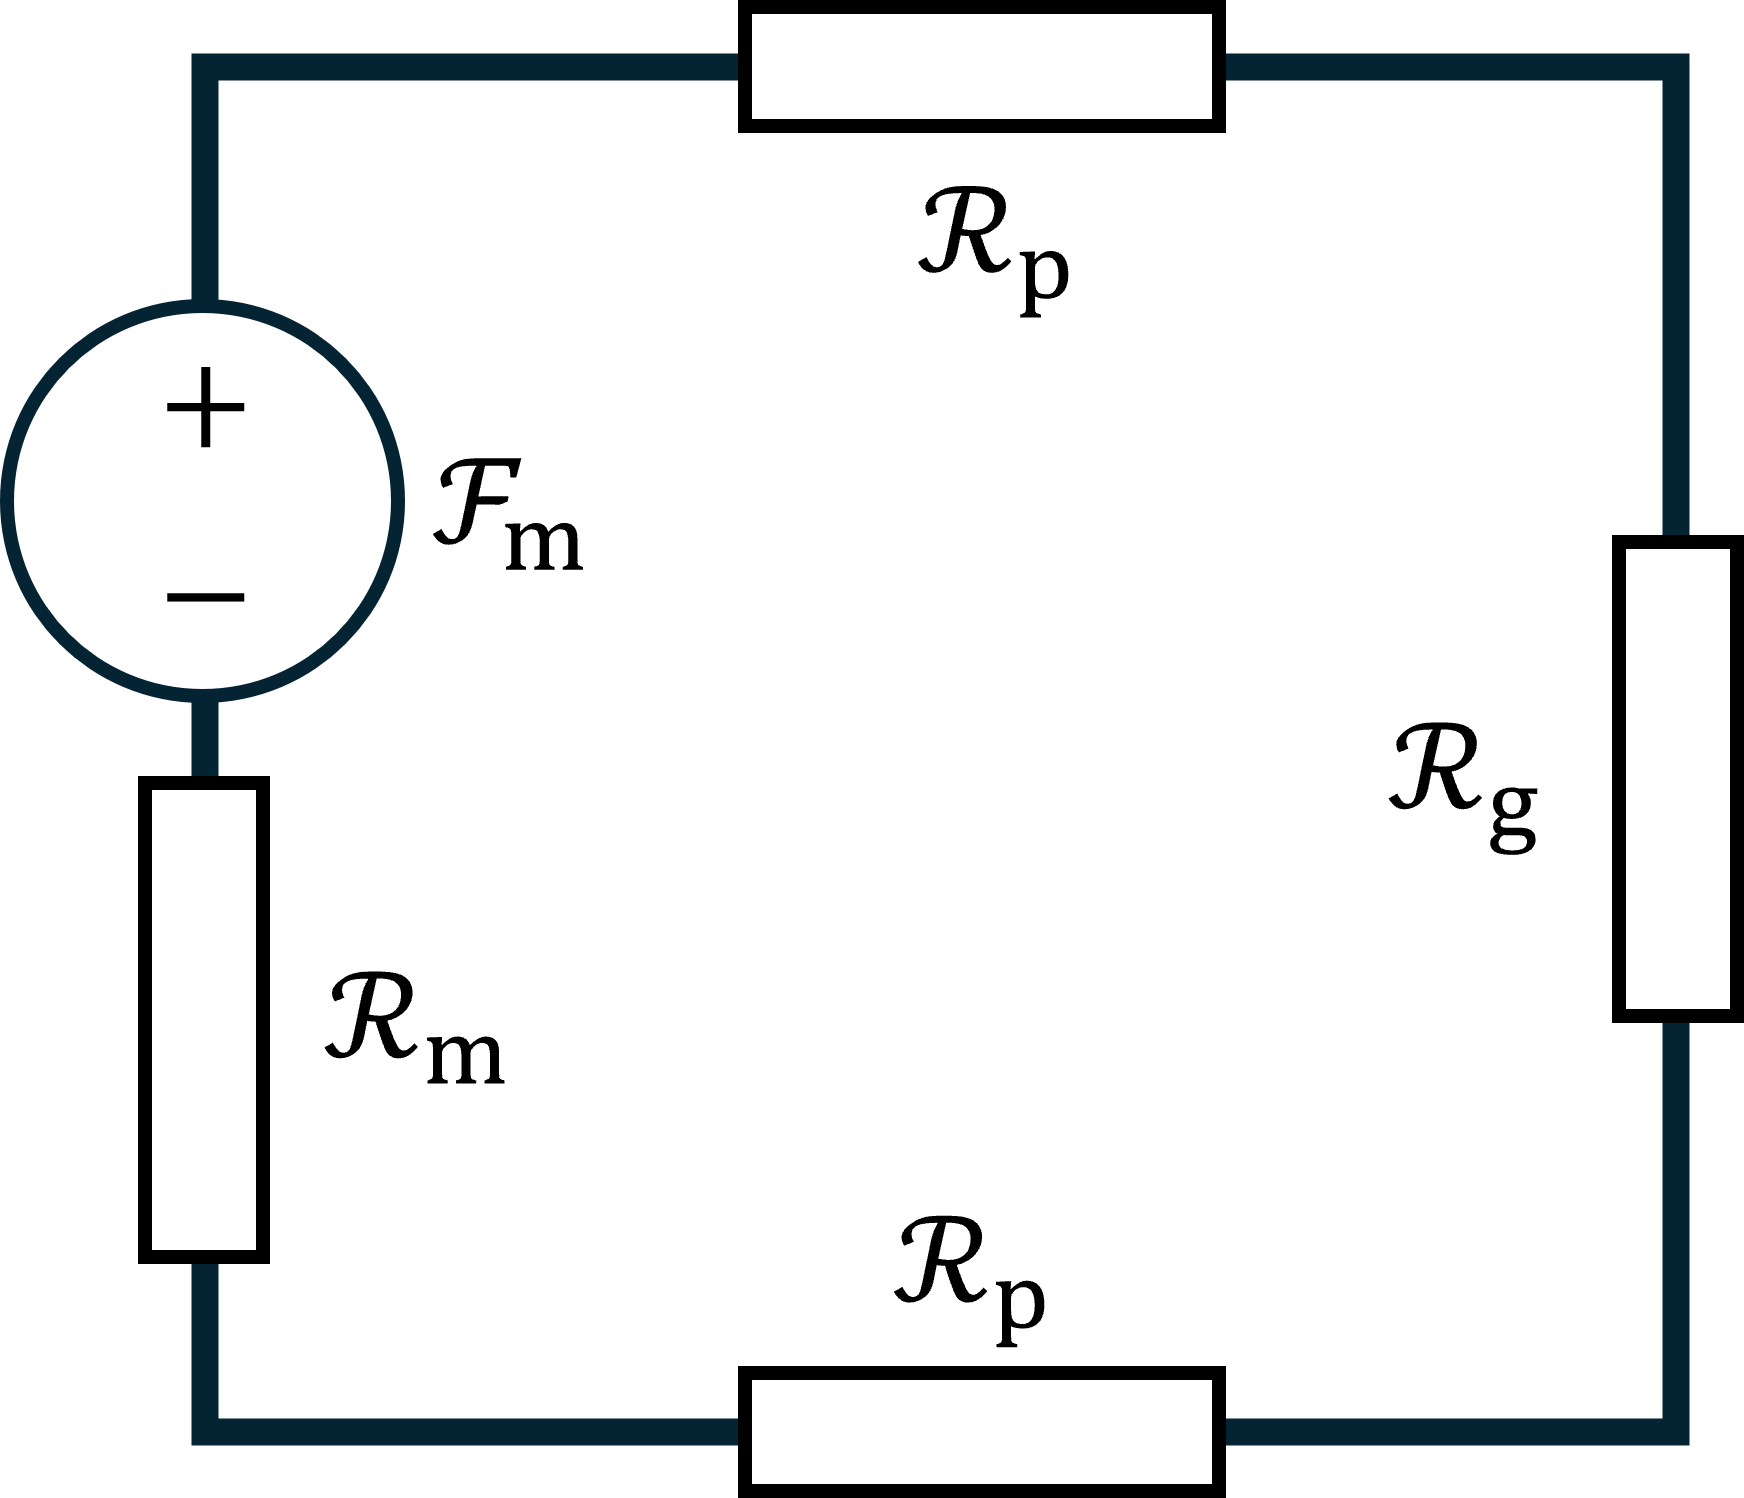
\includegraphics[width=\linewidth]{Images/magnetic_circuit_symbolic.png}
        \caption{}
        \label{fig:magnetic_circuit_b}
    \end{subfigure}
    \caption{Illustratie van het magnetisch circuit equivalent aan dat van de lens. De gap veroorzaakt een reluctantie die ervoor zorgt dat het oppervlakteveld $B_m$ van de magneet kleiner wordt dan haar remanent veld $B_r$. Dit kunnen we wiskundig beschrijven door de analogie te maken met elektrische circuits, waarbij de magneet een bron van magnetomotorische kracht, en de gap een reluctantie voorstellen.}
    \label{fig:magnetic_circuit}
\end{figure}

De totale reluctantie van het circuit kan berekend worden uit\footnote{Hierbij benaderen we de permeabiliteit van lucht $\mu_{lucht}\approx\mu_0$.}:
\begin{align}
    & \mathcal{R}_{tot}= \int_\Gamma \frac{dl}{\mu(l)A(l)} = \mathcal{R}_{m} + 2\mathcal{R}_{p} + \mathcal{R}_{g}\\
    &= \int_{magneet}\frac{dl}{\mu_{m}A(l)} + 2\int_{polepiece}\frac{dl}{\mu_{p}A(l)} + \int_{gap}\frac{dl}{\mu_{0}A(l)}
\end{align}
De permeabiliteit van de polepieces $\mu_p$ is heel groot, dus is $\mathcal{R}_{p}\approx 0$ en verwaarloosbaar. We kunnen de reluctantie van de magneet en de gap nu expliciet uitschrijven in functie van de lensparameters, met $A_m = \pi\left(R_{2, m}^2-R_{1, m}^2\right)$ de oppervlakte van de ringmagneet en $A_g = \pi\left(R_{2}^2-R_{1}^2\right)$ de oppervlakte van de polepieces aan de gap. Hierbij verwaarlozen we het naar buiten buigen van de veldlijnen, wat $A_g$ iets groter zou maken. Dit effect is echter klein in verhouding met de oppervlakte van de polepieces. De totale reluctantie wordt dan:
\begin{equation}
    \mathcal{R}_{tot}=\frac{d_m}{\mu_m A_m}+\frac{d_g}{\mu_0 A_g}
\end{equation}
Waarbij $d_m$ en $d_g$ respecievelijk de dikte van de magneet en van de gap voorstellen. De magnetomotorische kracht van de magneet wordt gegeven door\color{red} REFERENTIES? \color{black}:
\begin{equation}
    \mathcal{F}_m = H_c d_m = \frac{B_r d_m}{\mu_m }
\end{equation}
Hierbij geldt er dat $B_r = \mu_m H_c$ zolang de polepieces niet gesatureerd raken en de $B-H$ curve lineair blijft. Nu kunnen we de totale flux doorheen het circuit berekenen:
\begin{equation}
    \Phi = B_r\frac{d_m}{\mu_m  \left(\frac{d_m}{\mu_m A_m}+\frac{d_g}{\mu_0 A_g}\right)}=B_r\frac{A_m}{\left(1+\frac{\mu_m d_g A_m}{\mu_0 d_m A_g}\right)}
\end{equation}
Het magnetisch veld aan het oppervlak grenzend aan de gap kunnen we dan berekenen door rekening te houden met de oppervlaktes van de polepieces $A_g$:
\begin{equation}
    B_g = \frac{\Phi}{A_g} = \frac{B_r}{\left(\frac{A_g}{A_m}+\frac{\mu_m d_g}{\mu_0 d_m}\right)}
\end{equation}
Dit kunnen we nu gebruiken om de juiste waarde voor $\sigma_M$ te vinden. Voor een oneindige holomeen geladen vlakke plaat zou er gelden dat $H = \sigma_m$ en dus dat $B = \mu_0 \sigma_M$. In ons geval geldt er dus dat:

\begin{equation}\label{eq:charge_density}
    \sigma_M = \frac{B_g}{\mu_0} = \frac{B_r}{\left(\mu_0\frac{A_g}{A_m}+\frac{\mu_m d_g}{d_m}\right)}
\end{equation}

De volledige analytische uitdrukking van het magnetisch veld op de optische as van de lens verkrijgen we door de ladingsdichtheid in te vullen in vergelijking \ref{eq:2_annula} en wordt dus gegeven door de volgende vergelijking:\small
\begin{equation}\label{eq:analytical_B_field_final}
    B(z) = \frac{B_r}{\left(\frac{A_g}{A_m}+\frac{\mu_m d_g}{\mu_0 d_m}\right)}
    \begin{aligned}[t]
        &\left[ \frac{z+\frac{d_g}{2}}{2}\left(\frac{1}{\sqrt{\left(z+\frac{d_g}{2}\right)^2+R_1^2}}-\frac{1}{\sqrt{\left(z+\frac{d_g}{2}\right)^2+R_2^2}}\right)\right.\\
        &\left.- \frac{z-\frac{d_g}{2}}{2}\left(\frac{1}{\sqrt{\left(z-\frac{d_g}{2}\right)^2+R_1^2}}-\frac{1}{\sqrt{\left(z-\frac{d_g}{2}\right)^2+R_2^2}}\right)\right]
    \end{aligned}
\end{equation}

% \begin{align}\label{eq:analytical_B_field_final_alternative}
%     B(z) & = \frac{B_r}{\left(\frac{A_g}{A_m}+\frac{\mu_m d_g}{\mu_0 d_m}\right)}\sum_{\pm}\pm\frac{\zeta_{\pm}}{2}\left(\frac{1}{\sqrt{\zeta_{\pm}^2+R_1^2}}-\frac{1}{\sqrt{\zeta_{\pm}^2+R_2^2}}\right)\\
%     \zeta_{\pm} & = z \pm \frac{d_g}{2}
% \end{align}

\section{Implementatie van paraxiale bewegingsvergelijking in Python}
Met de analytische uitdrukking voor het magnetisch veld kunnen we de paraxiale bewegingsvergelijking oplossen om uiteindelijk de lenseigenschappen van de lens te gaan voorspellen. Ter herinnering, de paraxiale bewegingsvergelijking wordt gegeven door:
\begin{equation}\label{eq:paraxialevgl_rel_H54}
    \frac{d^2r}{dz^2}+\frac{\eta^2B(z)^2}{4V}r=0
\end{equation}
Hoewel de vergelijking er niet al te complex uit ziet, is het helemaal niet triviaal om ze voor eender welk magnetisch veld exact op te lossen. Slechts in enkele gevallen is er een analytische oplossing in gesloten vorm gekend. Een voorbeeld hiervan is \textit{Glaser's bell-shaped field}:
\begin{equation}\label{eq:Glasers_field}
    B(z) = \frac{B_0}{1+\frac{z^2}{a^2}}
\end{equation}
De oplossing van vergelijking \ref{eq:paraxialevgl_rel_H54} kan voor dit veld worden uitgedrukt met goniometrische functies \cite{PWHawkes}. Het magnetisch veld kan ook benaderd worden door een constant veld:
\begin{equation}\label{eq:constant_field}
    B(z) = 
    \begin{cases}
        B_0 & z<\left|\frac{d}{2}\right|\\
        0 & z>\left|\frac{d}{2}\right|\\
    \end{cases}
\end{equation}
In dat geval heleidt vergelijking \ref{eq:paraxialevgl_rel_H54} zich tot een harmonische oscillator in de lens. Echter, beide velden zijn niet fysisch, en slechts benaderingen van werkelijke magnetische velden. Figuur \ref{fig:fields_comparison} geeft een vergelijking tussen deze twee velden en ons afgeschatte veld.
\begin{figure}[H]
    \centering
    \begin{subfigure}[b]{0.3\linewidth}
        \centering
        
\includegraphics[width=\linewidth]{Images/Glasers_B_field.png}
        \caption{}
        \label{fig:fields_comparison_a}
    \end{subfigure}
    \hfill
    \begin{subfigure}[b]{0.3\linewidth}
        \centering
        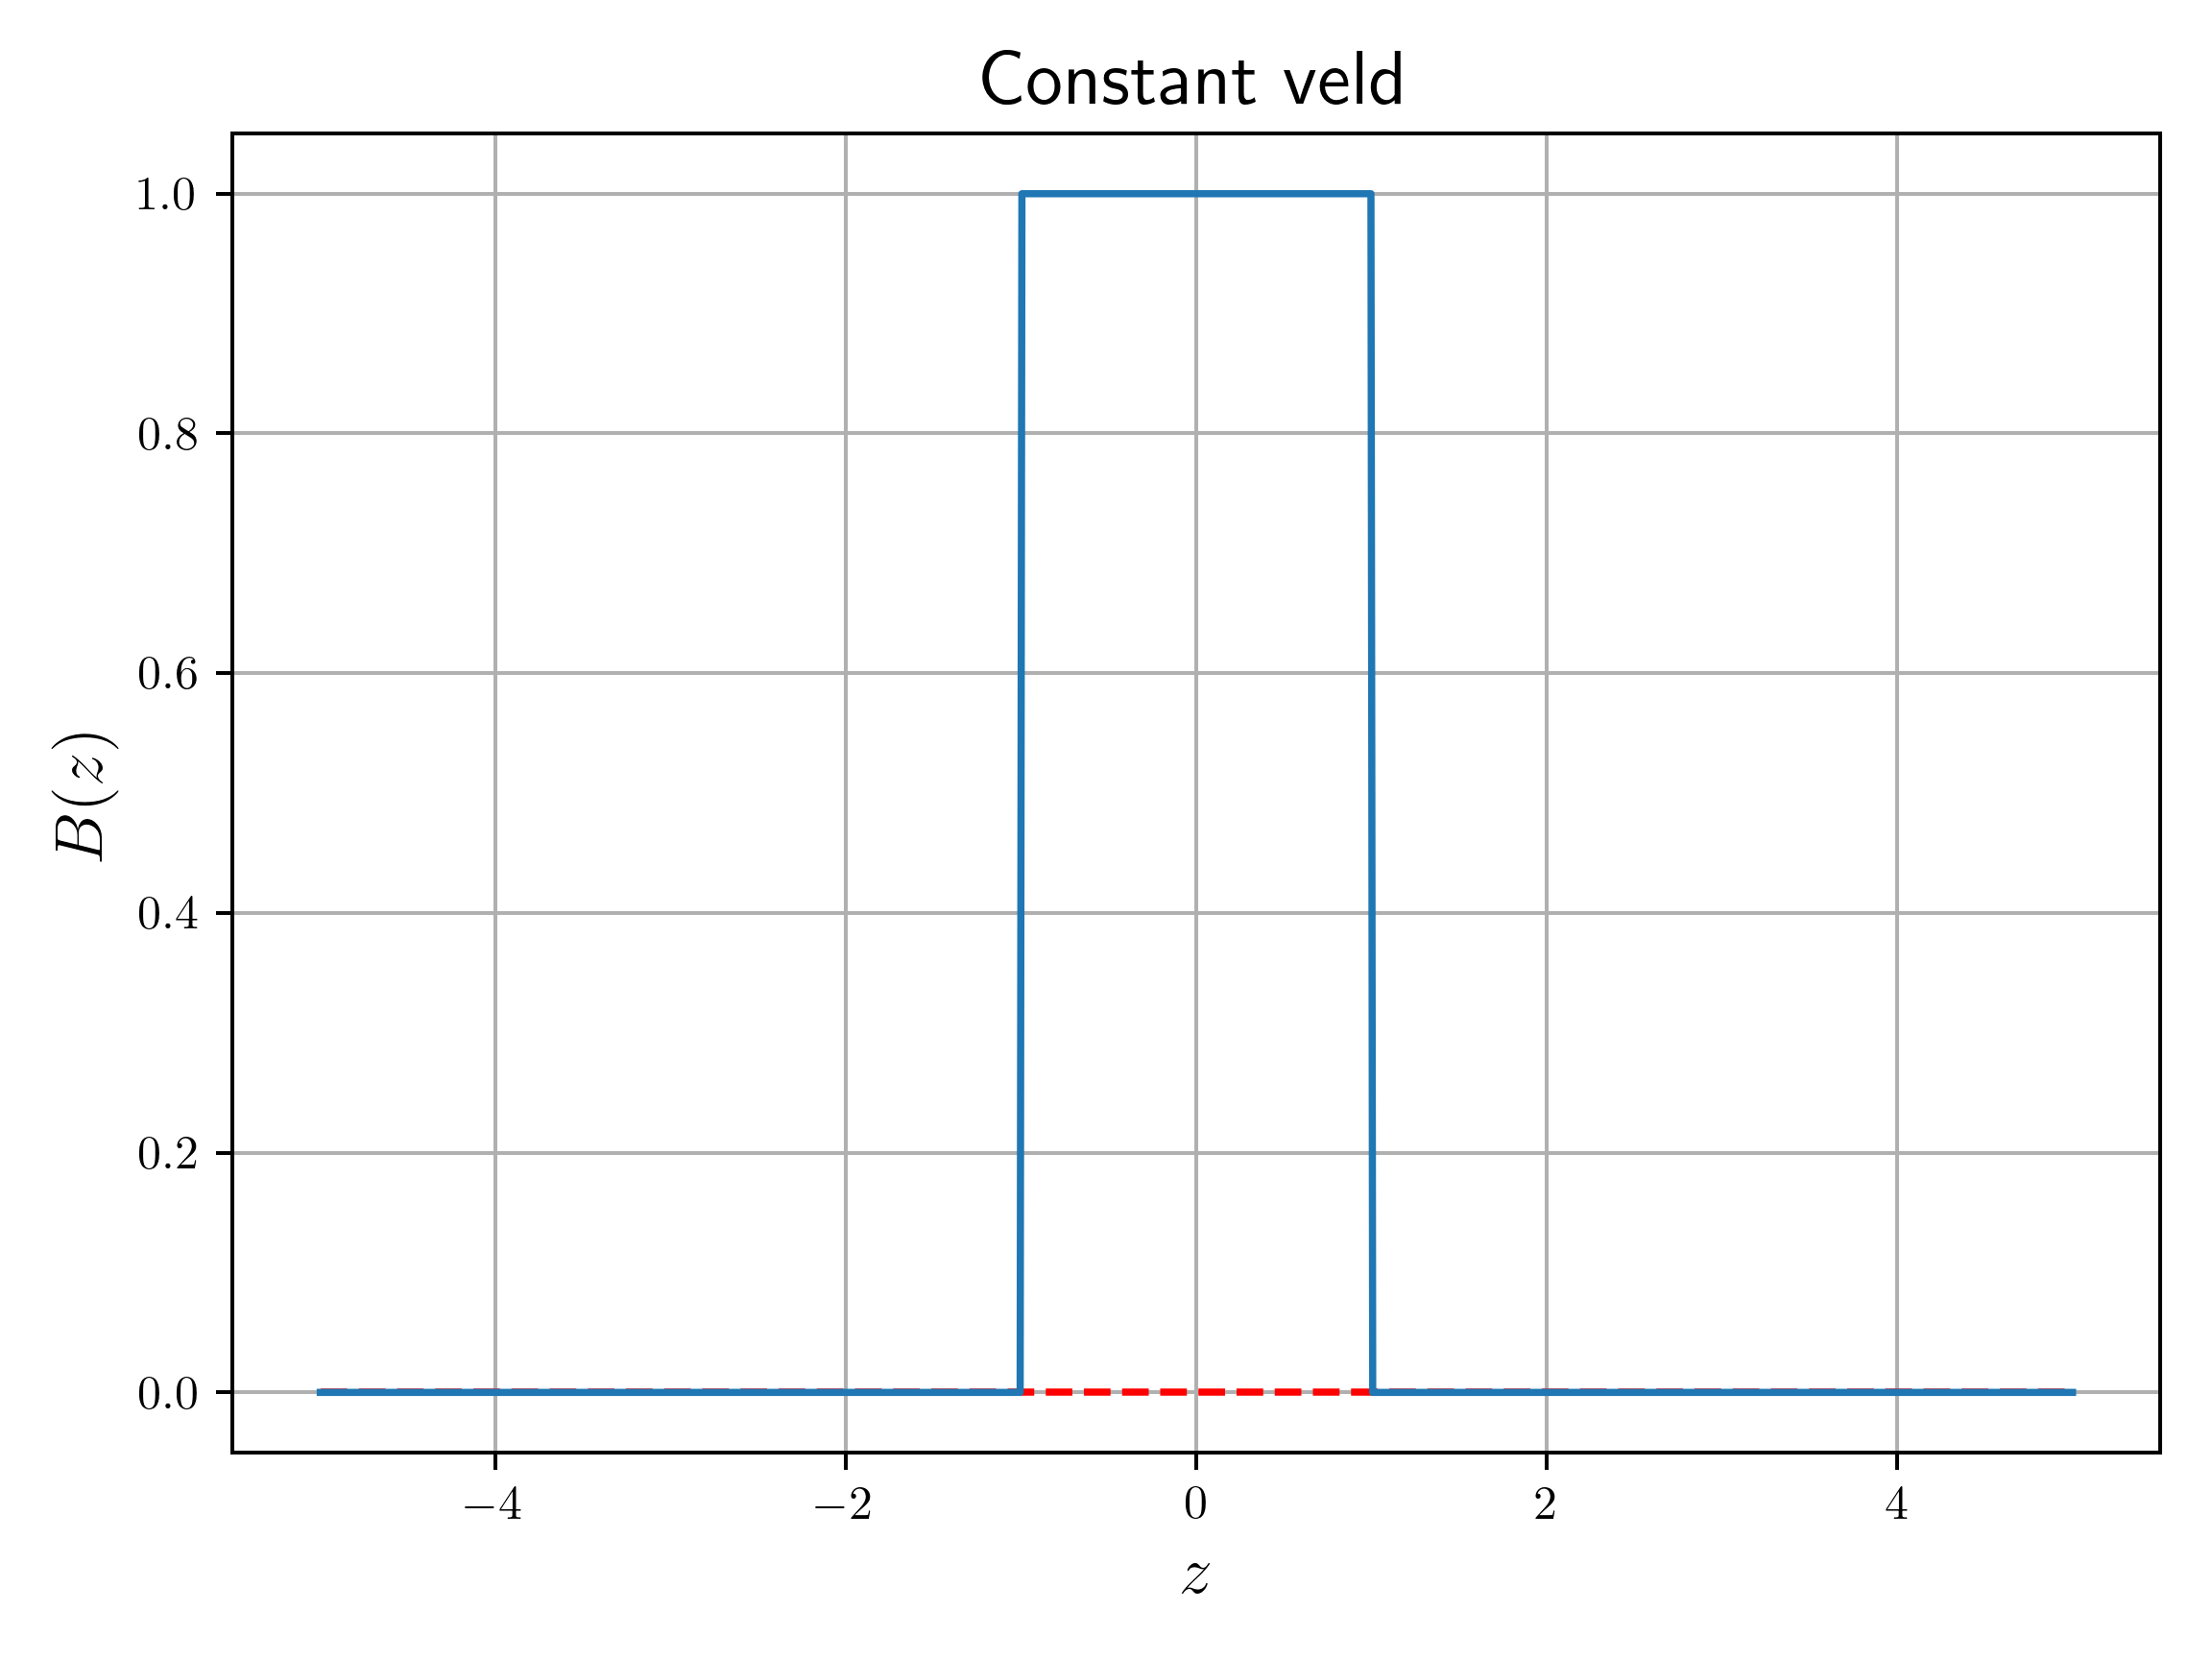
\includegraphics[width=\linewidth]{Images/Constant_B_field.png}
        \caption{}
        \label{fig:fields_comparison_b}
    \end{subfigure}
    \hfill
    \begin{subfigure}[b]{0.3\linewidth}
        \centering
        
\includegraphics[width=\linewidth]{Images/Actual_B_field.png}
        \caption{}
        \label{fig:fields_comparison_c}
    \end{subfigure}
    \caption{Vergelijking tussen twee velden (Glaser's field en constant veld) waarvoor de paraxiale bewegingsvergelijking analytisch oplosbaar is en ons analytisch afgeschat veld. Het Glaser's field is gelijkaardig, maar heeft een bredere piek en valt trager af dan ons afgeschatte veld. Dit geeft een dikkere lens, wat ongewenst is.}
    \label{fig:fields_comparison}
\end{figure}
We zien dat het Glaser's field een goede benadering zou geven, maar de piek in het magnetisch veld is breder het veld vlakt trager af dan het veld van onze lens. Om accurate voorspellingen van onze lens te kunnen maken, kiezen we er daarom voor om de paraxiale beweginsvergelijking numeriek op te lossen en hieruit de lenseigenschappen te bepalen. Dit laat ons ook toe om later Monte Carlo simulaties van experimentele opstellingen uit te voeren, zodat we kunnen inschatten welke opstellingen ons bruikbare resultaten kunnen geven.\\

We maken hiervoor gebruik van Python. We schreven een klasse waarin we de parameters van de lens (binnen- en buitenstralen, diktes van de gap en magneet, sterkte van de magneet etc.) en de opstelling in de microscoop (afstanden tussen voorwerp en lens, versnelspanning etc.) kunnen instellen. Met deze parameters kunnen we dan het analytische veld berekenen en plotten. Dit laat ons toe om snel en efficient te bepalen hoe het magnetisch verandert in functie van de parameters. Dit zal in meer detal worden besproken in het volgende hoofdstuk.\\

Om de paraxiale bewegingsvergelijking op te lossen, gebruiken we de solve\_ivp functie van de scipy.integrate bibliotheek. Het objectvlak $z_0$ kunnen we naar wens instellen, en we gebruiken een 8ste orde Runge-Kutta methode (DOP853) om de twee lineair onafhankelijke oplossingen $g$ en $h$ te berekenen. De oplossing $g(z)$, waarvoor geldt dat $g(z_0)=1$ en $g'(z_0)=0$, kunnen we dan gebruiken om de lenseigenschappen te berekenen. Ten eerste kijken we in welk vlak de twee asymtoten van $g(z)$, de object en beeld asymtotische bundels, elkaar snijden. Dit vlak is het achterste/beeld hoofdvlak van de lens $z_{Pi}$. Ten tweede kijken we waar de beeld asymtotische bundel de symmetrie-as van de lens snijdt. Alle parallel bewegende elektronen zullen door dit punt passeren, dus dit is het brandpunt in het focusvlak $z_{Fi}$ van de lens. De brandpuntsafstand kunnen we dan berekenen uit $f=z_{Fi}-z_{Pi}$. Door de symmetrie van het magnetisch veld kunnen we het object beeldvlak en het object focusvlak vinden uit $z_{Po}=-z_{Pi}$ en $z_{Fo}=-z_{Fi}$, Figuur \ref{fig:setup_1} toont een voorbeeld van een numerieke oplossing van $g$. In dit geval vinden we een brandpuntsafstand van $f=11.48\mathrm{mm}$ en bevindt het beeld hoofdvlak zich op $z_{Pi}=0.48\mathrm{mm}$ van het midden van de lens.

\begin{figure}[H]
    \centering
    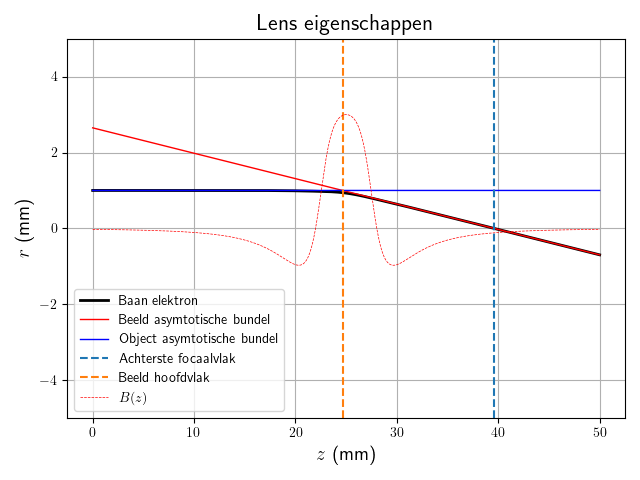
\includegraphics[width=0.6\linewidth]{Images/setup_1.png}
    \caption{Plot van numerieke oplossing van de paraxiale bewegingsvergelijking. De object en beeld asymptotische bundels snijden elkaar in het beeld hoofdvlak, en de beeld asymtotische straal snijdt de symmetrie-as in het achterste focaalvlak van de lens. Deze opstelling heeft de volgende parameters: $R_1=1.5\mathrm{mm},R_2=5\mathrm{mm},d=5\mathrm{mm}, B_g=0.447\mathrm{T},\Phi=30\mathrm{KeV}$.}
    \label{fig:setup_1}
\end{figure}

Eens we de twee lineair onafhankelijke oplossingen hebben berekend, is het mogelijk om de baan van eender welk elektron af te beelden door een lineaire combinatie van de twee oplossingen te maken. Op deze manier kunnen we stralingsdiagrammen zoals Figuur \ref{fig:setup_2}, waarbij we de lens van de voorgaande figuur hebben gebruikt om een vergroting van $M=5$ te krijgen. We tekenen op de figuur de drie hoofdstralen: de straal die door het midden van de lens gaat, en de straal die door het voorste brandpunt gaat. Deze drie kruisen elkaar in 1 punt achter de lens, waar het beeld gevormd wordt. Merk ook op dat de straal die door het midden van de lens gaat niet wordt afgebogen, zoals men zou verwachten.

\begin{figure}[H]
    \centering
    
\includegraphics[width=0.6\linewidth]{Images/setup_2.png}
    \caption{Voorbeeld van beeldvorming met een permanente magneetlens. We beschouwen hier de drie hoofdstralen: de straal die door het achterste brandpunt gaat, de straal die door het midden van de lens gaat, en de straal die door het voorste brandpunt gaat. In dit geval krijgen we een magnificatie $M=5$.}
    \label{fig:setup_2}
\end{figure}

\section{Lensontwerp}
Nu we in staat zijn om de banen van elektronen door het magnetisch veld van een lens te simuleren, kunnen de parameters van de lens gaan optimaliseren om een geschikte dunne lens te maken. Hierbij moeten we rekening houden met het volgende:
\begin{enumerate}
    \item We willen liefst een dunne lens, dus willen we $z_{Pi}\approx0$. Dit betekent dat dat $B(z)$ een smalle piek moet vertonen.
    \item We willen een lens die we in de MIRA microscoop kunnen gebruiken. Concreet betekent dit dat we een focale lengte willen die rond de $5-10\mathrm{mm}$ ligt. Hiervoor moet $\sigma_M$ voldoende groot zijn, en moet $R_1$ voldoende klein zijn zodat de ladingen zich niet te ver van de opticshe as bevinden.
    \item De verhouding tussen het remanent veld van de magneet en het werkelijke veld in de magneet wordt gegeven door:
    \begin{equation}
        \frac{B_m}{B_r} = \frac{1}{1+\frac{\mu_m A_m d_g}{\mu_0 A_g d_m}}
    \end{equation}
    Hoe groter het demagnetiserend veld dat het remanent veld tegenwerkt, hoe kleiner deze verhouding. Echter, bij een bepaald kritiek veld passeren we de \"elleboog\" van de hysteresiscurve van het materiaal waardoor de permanente magneet zal beginnen demagnetiseren. Dit effect willen we vermijden om te voorkomen dat de sterkte van de magneet, en dus ook de lens doorheen de tijd zal afnemen.

\end{enumerate}


\begin{figure}[H]
    \centering
    % --- First Row ---
    \begin{subfigure}[b]{0.45\linewidth}
        \centering
        
\includegraphics[width=\linewidth]{Images/variable_R_1.png}
        \caption{}
        \label{fig:variable_R_1}
    \end{subfigure}
    \hfill
    \begin{subfigure}[b]{0.45\linewidth}
        \centering
        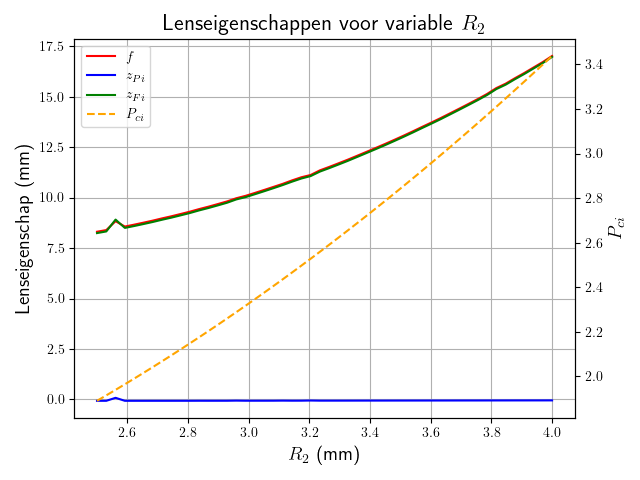
\includegraphics[width=\linewidth]{Images/variable_R_2.png}
        \caption{}
        \label{fig:variable_R_2}
    \end{subfigure}

    \vspace{0.5cm} % Adds vertical spacing between rows

    % --- Second Row ---
    \begin{subfigure}[b]{0.45\linewidth}
        \centering
        
\includegraphics[width=\linewidth]{Images/variable_d.png}
        \caption{}
        \label{fig:variable_d}
    \end{subfigure}
    \hfill
    \begin{subfigure}[b]{0.45\linewidth}
        \centering
        
\includegraphics[width=\linewidth]{Images/variable_B_r.png}
        \caption{}
        \label{fig:variable_B_r}
    \end{subfigure}

    \caption{Plots van lenseigenschappen en reluctantieterm in functie van de geometrie van de lens. Deze plots geven een geod beeld van hoe de parameters aangepast kunnen worden om de lenseigenschappen naar wens te optimaliseren. Naast de reluctantieterm moet er ook rekening gehouden worden met de maximale fluxdichtheid in de polepieces, welke niet te hoog mag zijn om saturatie-effecten te voorkomen.}
    \label{fig:grid_2x2}
\end{figure}


\section{Monte Carlo simulatie van experiment}

\section{Experimentele bepaling focale lengte}

\chapter{Besluit}

\bibliographystyle{alpha}
\bibliography{bibliography}

\end{document}


\endinput
%%
%% End of file `uantwerpenbamathesis-example.tex'.
